%%----------------------------------------------------------------------
\title*{Project CASSIA\\
   --- Framework for Exhaustive and Large-scale Social Simulation ---}
\author{%
   Itsuki Noda,
   Yohsuke Murase,
   Nobuyasu Ito,
   Kiyoshi Izumi,
   Hiromitsu Hattori,
   Tomio Kamada, 
   Hideyuki Mizuta, and
   Mikio Takeuchi}
\institute{%   
   Itsuki Noda \at AIST, 1-1-1 Umezono, Tsukuba, Japan, \email{i.noda@aist.go.jp} \and
   Yohsuke Murase \at RIKEN Center for Computational Science, 7-1-26, Minatojima-minami-machi, Chuo-ku, Kobe, Japan, \email{yohsuke.murase@gmail.com} \and
   Nobuyasu Ito \at Univ. Tokyo \& Riken \and
   Kiyoshi Izumi \at Univ. Tokyo \and
   Hiromitsu Hattori \at Ritsumei Univ. \and
   Tomio Kamada \at Kobe Univ. \and
   Hideyuki Mizuta \at IBM \and
   Mikio Takeuchi \at IBM}
\maketitle
%%----------------------------------------------------------------------

%%----------------------------------------------------------------------
\abstract*{%
  Project CASSIA (Comprehensive Architecture of Social Simulation for
  Inclusive Analysis) aims to develop a framework to administer to
  execute large-scale multiagent simulations exhaustively to analyze
  socially interactive systems. The framework will realize engineering
  environment to design and synthesize social systems like traffics,
  economy and politics.
}
%%----------------------------------------------------------------------

%%----------------------------------------------------------------------
\section{Overview}
\label{s:Overview}
%% - - - - - - - - - - - - - - - - - - - - - - - - - - - - - - - - - - -

Project CASSIA (Comprehensive Architecture of Social Simulation for
Inclusive Analysis) aims to develop a framework to administer to
execute large-scale multiagent simulations exhaustively to analyze
socially interactive systems. The framework will realize engineering
environment to design and synthesize social systems like traffics,
economy and politics.

The purpose of multi-agent social simulation is to provide
tools to design social systems.
It is impossible or quite difficult to carry out experiments
of social phenomena in the real world 
by the similar way as experiments in physics or chemistry.
Therefore, computational social simulations are indispensable means
for social science.

Fortunately,
progress of computational power has a potential to realize wider applications of
computer simulation not only in physical phenomena but also in social 
problems.
High performance computing (HPC) has been enabling several simulation researches
on large-scale weather, molecular dynamics, structures and architectures, and
disasters.
In addition to these physical phenomena,
recently,
social phenomena like economics, traffics, or information flow on
networks
attract many attentions as applications of HPC.

In order to make such social simulations on HPC
available for wide-range users,
the CASSIA framework consists of:
\begin{itemize}
  \item
    MASS Planning Module: a manager module conducts effective
    execution plans of simulations among massive possible conditions
    according to available computer resources.
  \item
    MASS Parallel Middleware: an execution middleware provides
    functionality to realize distributed multi-agent simulation on
    many-core computers.
\end{itemize}

%%++++++++++++++++++++++++++++++++++++++++++++++++++++++++++++++++++++++
\begin{figure}
  \centering
  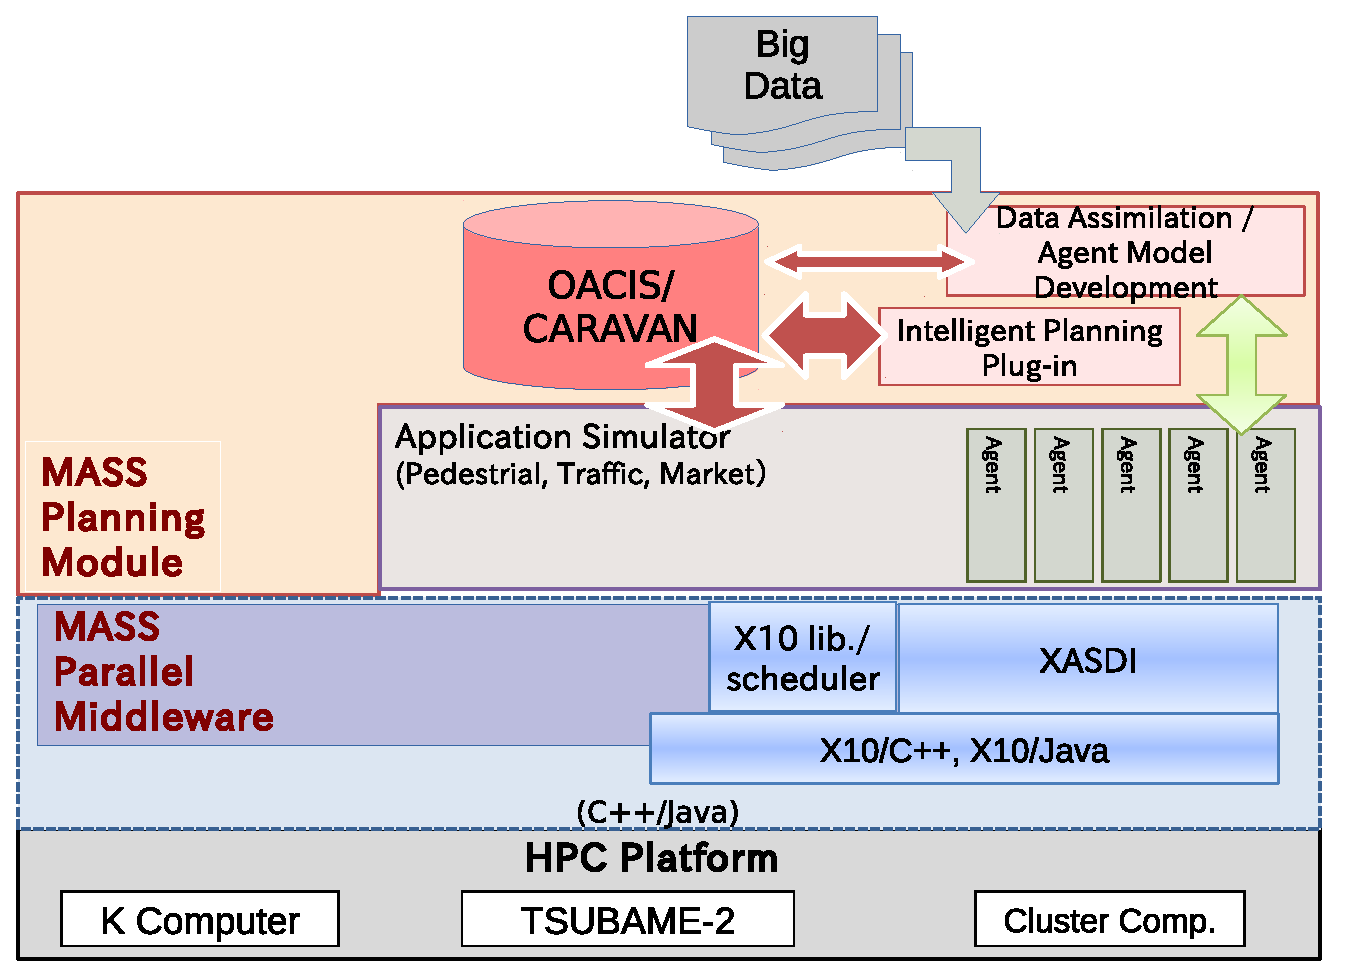
\includegraphics[width=.8\linewidth]{Figs.noda/figure-01.framework.eps}
  \caption{Cassia Framework}
  \label{fig:Figs.noda/figure-01.framework.eps}
\end{figure}
%%++++++++++++++++++++++++++++++++++++++++++++++++++++++++++++++++++++++



%%----------------------------------------------------------------------
\section{MASS Planning Module}
\label{s:MASS Planning Module}
%% - - - - - - - - - - - - - - - - - - - - - - - - - - - - - - - - - - -

(Murase, Ito)

OACIS (Organizing Assistant for Comprehensive and Interactive
Simulations) is a job management software for large-scale
simulations. It controls a large number of simulation jobs executed in
various remote servers, keeps these results in an organized way, and
manages the analyses on these results.

%%++++++++++++++++++++++++++++++++++++++++++++++++++++++++++++++++++++++
\begin{figure}
  \centering
  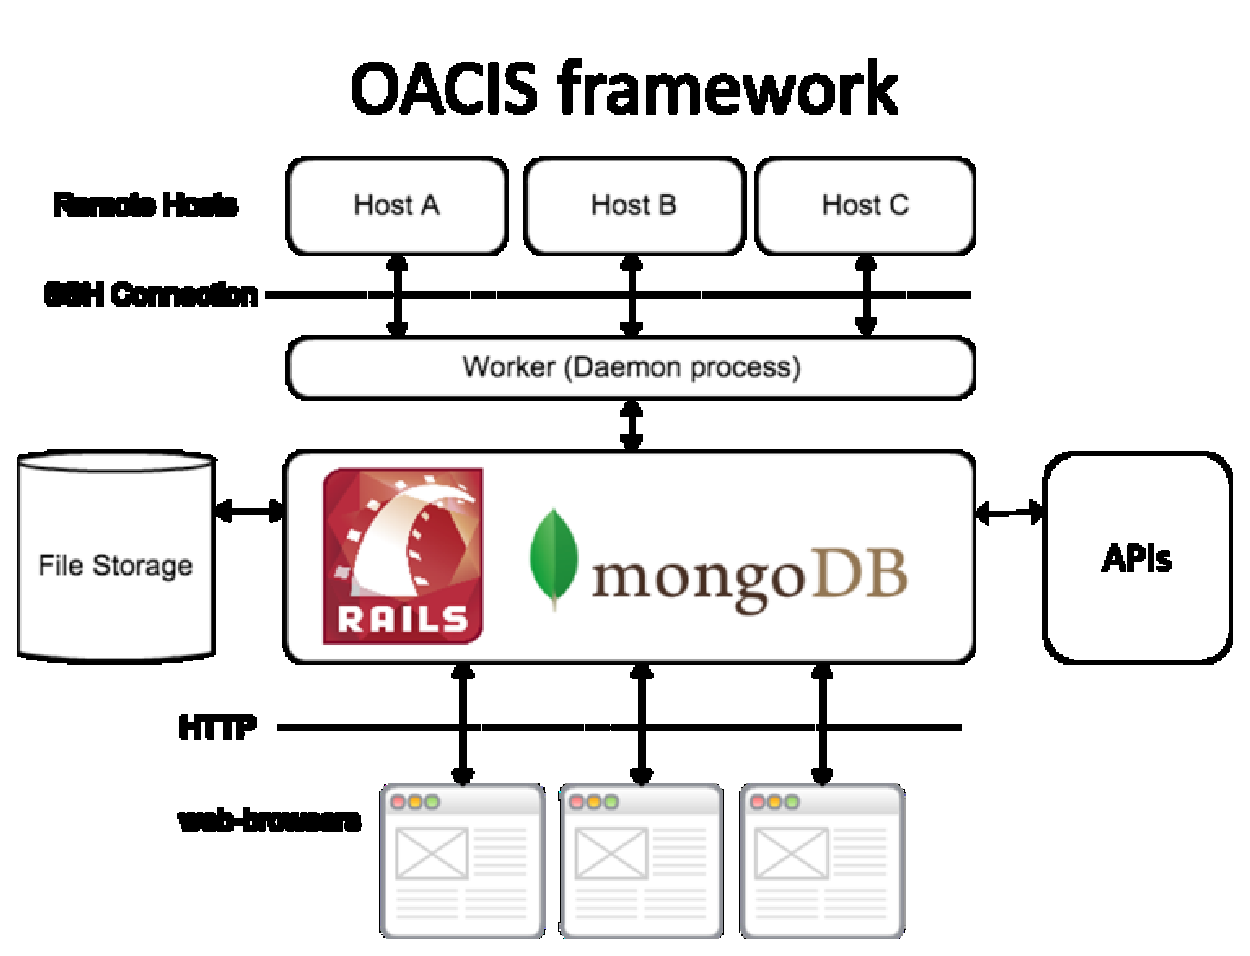
\includegraphics[width=.8\linewidth]{Figs.noda/figure-02.oacis.eps}
  \caption{OACIS}
  \label{fig:Figs.noda/figure-02.oacis.eps}
\end{figure}
%%++++++++++++++++++++++++++++++++++++++++++++++++++++++++++++++++++++++

CARAVAN provides more powerful scalability for exhaustive
simulation. These functionalities are especially beneficial for the
complex simulation models having many parameters for which a lot of
parameter searches are required.

%%++++++++++++++++++++++++++++++++++++++++++++++++++++++++++++++++++++++
\begin{figure}
  \centering
  
\includegraphics[width=.8\linewidth]{Figs.noda/figure-03.caravan.eps}
  \caption{CARAVAN}
  \label{fig:Figs.noda/figure-03.caravan.eps}
\end{figure}
%%++++++++++++++++++++++++++++++++++++++++++++++++++++++++++++++++++++++


%%----------------------------------------------------------------------
\section{MASS Parallel Middleware}
\label{s:MASS Parallel Middleware}
%% - - - - - - - - - - - - - - - - - - - - - - - - - - - - - - - - - - -

%%--------------------------------------------------
\subsection{X10 Extentions and Plham}
\label{ss:X10 Extentions and Plham}
%% - - - - - - - - - - - - - - - - - - - - - - - - -

To realize distributed multi-agent simulation on large scale distributed computers,
we developed parallel middleware on X10~\cite{x10},
which is an object-oriented parallel programming language developed by IBM.
X10 adopts partitioned global address space (PGAS) model,
and features asynchronous and fork-join-style programs.
Using X10 and our parallel middleware, we developed Plham~\cite{toriiPlham,arob17plham}, 
a platform for large-scale and high-frequency artificial
market simulation.
In this section, we first summarize the design and implementation of Plham to enable 
large-scale and high-frequency artificial markte simulation.
Then we show two libraries, 
a distributed collection library and
a global load balancing library with multi-stage facility~\cite{glb2m}, 
that are designed for large-scale multi-agent simulations.

Artificial market agent-based simulations have potential to be a strong tool for studying rapid and large market fluctuation and designing Financial regulations.
High-frequency traders, that exchange multiple assets simultaneously within a millisecond,
is said to be a cause of rapid and large market fluctuation.
% Plham is designed to allow users to define their simulation models without parallel computing expertise.
Plham enables modeling financial markets
composed of various brands of assets and a large number of agents trading on a short timescale.
The design feature of Plham is the separation
of artificial market models (simulation models) from their execution (Figure~\ref{fig:Figs.kamada/plham}).
The primary components of a simulation model are 'agents' and 'markets' as shown in (a).
The term \textit{agent} is used to represent a trader, including high-frequency traders.
The term \textit{market} is used to represent a system or place where agents can buy or sell a specific asset (here, we assume one market is for one asset).
Some type of asset depends on a collection of assets and is itself a tradable financial instrument (e.g., index-futures, exchange-traded funds). 
Users can employ ready-made agent/market classes provided by Plham or define
their original ones by extending these classes,
and construct their simulation models without parallel computing expertise.

%%++++++++++++++++++++++++++++++++++++++++++++++++++++++++++++++++++++++
\begin{figure}[t]
  \centering
  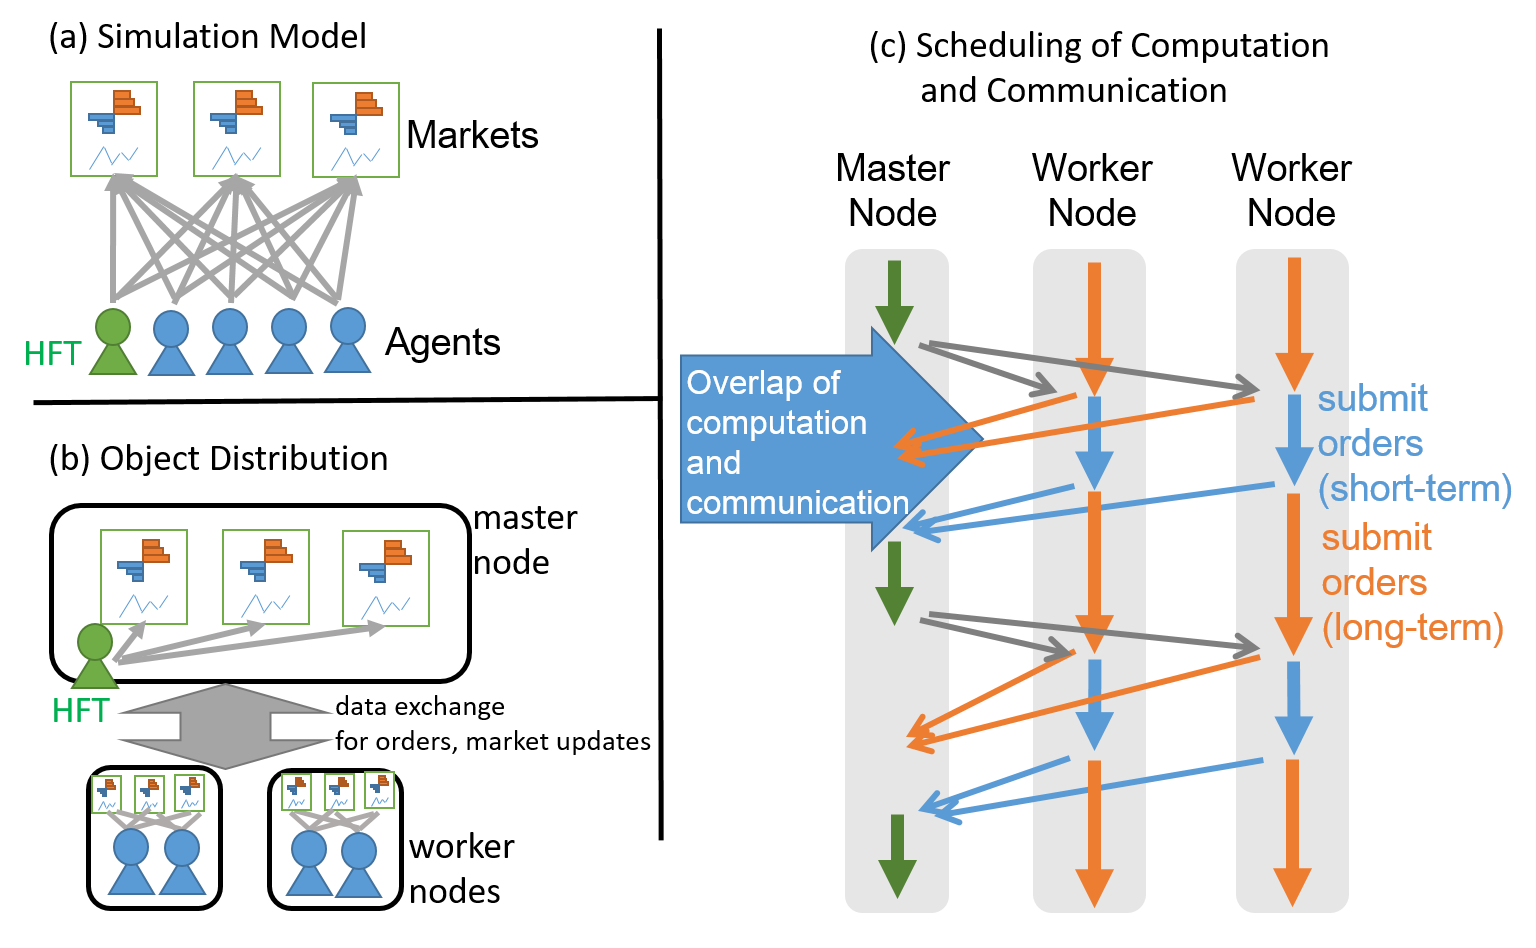
\includegraphics[width=.8\linewidth]{Figs.kamada/plham.png}
  \caption{Plham (Simulation Model and its Parallel Execution)}
  \label{fig:Figs.kamada/plham}
\end{figure}
%%++++++++++++++++++++++++++++++++++++++++++++++++++++++++++++++++++++++

Plham provides multiple runners that implement respective execution models.
To execute a parallel simulation, the users can employ a parallel runner implementing its parallel execution model that allocates agents over multiple computing nodes,
changes the scheduling frequency of agents, depending on the class of agents, and accepts delayed propagation of market information depending on the class.
In the current implementation, 
HFT agents are assigned at the master node, in which the order handling of the markets is processed,
and the computation for ordinal traders is executed at the worker nodes, as shown in Figure~\ref{fig:Figs.kamada/plham}~(b).
For large-scale simulations, nonHFT agents must be forced to make a decision by using delayed or out-of-date market information, whereas HFT agents are given access to latest or relatively up-to-date market information.

The current parallel runner allows concurrent execution of order submission and handling as shown in (c) to reduces CPU idle time at worker nodes and achieve simulation scalability.
To increase the parallelism of the simulation, the runner introduces three agent ranks: high-frequency traders, short-term traders, and long-term traders.
It then concurrently executes the order-submission stage of long-term traders and the order-handling stage of markets. 
In addition, it succeeded in overlapping communication and computation.
The scalability of the current parallel execution model was evaluated in weak-scaling to a maximum of 2048 computing nodes on the K computer~\cite{arob17plham}.
Plham is available as an open-source software under Eclipse Public License (http://github.com/crest-cassia/oacis).

To realize distributed multi-agent simulation on large scale distributed computers,
developers have to implement proper agent distribution, data transportation for agent communication, parallel execution of agent computation using multi-core CPUs, and efficient scheduling of respective components of computation and communication.
We developed a distributed collection library to easily manage
collection of object elements distributed over multiple computing nodes.
It offers methods for element relocation (communication) and data parallel processing for the elements (computation).
Our library provides a series of distributed collections, such as \texttt{DistCol[T], DistBag[T],} and
\texttt{DistMap[K,V]}, each of which manages a collection of objects that spreads over worker nodes.
Our library also prepared another type of distributed collection, \texttt{ColDist[T]}, that holds a list of objects
and allocates the cache proxies of the list at all worker nodes.
In the implementation of Plham, \texttt{ColDist} is used to manage markets and their proxies and
\texttt{DistCol} is used for agents.
Orders and contracted orders are stored into \texttt{DistBag} and \texttt{DistMap} and relocated at each calculation step.
Our library allows object transportation by using collective communication of MPI,
and the elapsed time for the communication can be reduced.
These classes also offers an asynchronous method,
\texttt{asyncEach},
that receive a function and apply it to all the local elements in the called node using thread pools.
Using these features, the overlapping of communication and computation in Plham was briefly described as shown in Figure~\ref{fig:Figs.kamada/middleware}~(a).

%%++++++++++++++++++++++++++++++++++++++++++++++++++++++++++++++++++++++
\begin{figure}
%    \centering
  \begin{minipage}{.33\textwidth}
    \begin{lstlisting}[basicstyle=\tiny, frame=single]
finish for (place in placeGroup)
 at (place) async {
  for(steps) {
    sCond = sAgents.eachAsync(..);
    if(!first) lOrders.relocate(..);
    sCond.await();
    lCond = lAgents.eachAsync(..);
    sOrders.relocate(..);
    if(master) markets.each(..); 
    markets.teamedBroadcast(..);
    contracted.relocate(..);
    lCond.await();
 }}
}
    \end{lstlisting}
  (a) Sample program of Distributed Collections
  \end{minipage}
  \hspace{4pt}
    \begin{minipage}{.3\textwidth}
      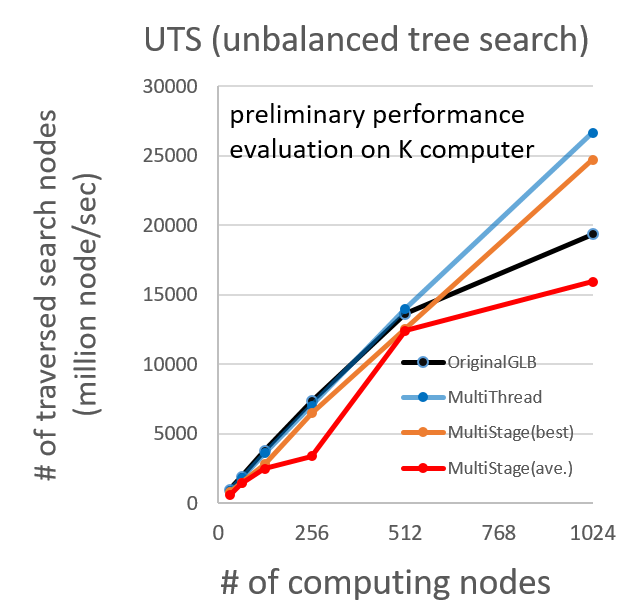
\includegraphics[width=\textwidth]{Figs.kamada/glbScale.png}
      (b) Performance evaluation of global load balancing 
    \end{minipage}
      \hspace{4pt}
        \begin{minipage}{.3\textwidth}
      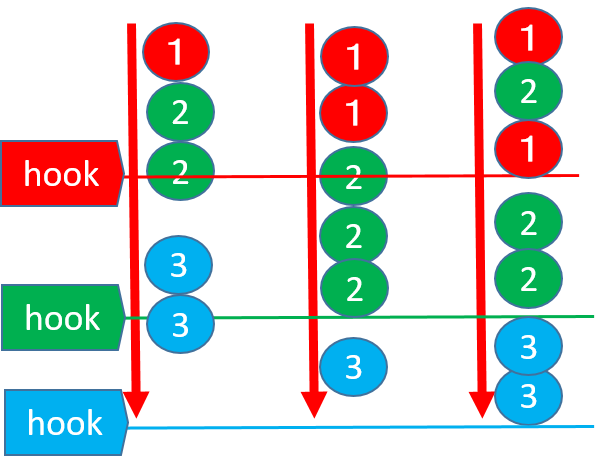
\includegraphics[width=\textwidth]{Figs.kamada/msGLB.png}
      (c) Multi-stage features for GLB
    \end{minipage}
  \caption{Parallel middleware for large-scale multi-agent simulations}
  \label{fig:Figs.kamada/middleware}
\end{figure}
%%++++++++++++++++++++++++++++++++++++++++++++++++++++++++++++++++++++++


We also conducted research on global load balancing for
 multi-agent simulation having multiple calculation steps.
Load balancing is a major concern in massively parallel computing.
X10 provides a global load balancing (GLB) library that 
shows high scalability over ten thousand CPU cores.
GLB features a lifeline-based scalable work-stealing algorithm.
Results of completed tasks are gathered by means of reduction operations.
We introduced a multithread design into GLB 
to allow efficient data sharing between CPU cores.
The multithread version showed high scalability than the original one (Figure~\ref{fig:Figs.kamada/middleware}~(b)).
In addition, we proposed a multistage mechanism for GLB to 
assign execution stages to tasks.
The system gives high priority to tasks that are assigned to earlier stages
and then proceeds with subsequent stage tasks (Figure~\ref{fig:Figs.kamada/middleware}~(c)).
When a computing node runs out of tasks at the earliest stage,
it requests tasks at the earliest stage from other nodes
and awaits responses by processing subsequent stage tasks.
When the system identifies the task termination at a certain stage,
it executes a reduction operation over nodes.
The multi-stage version has performance problems
that appear to be caused by network message scheduling or thread scheduling.
After fixing the problems,
we plan to introduce this dynamic load balancing features into our distributed collection library
to treat dynamic load imbalance of tasks.











%%--------------------------------------------------
\subsection{XASDI}
\label{ss:XASDI}
%% - - - - - - - - - - - - - - - - - - - - - - - - -

In this section, we describe the overview of X10-based Agent Simulation on Distributed Infrastructure (XASDI).
This framework is published as an open source software (\url{https://github.com/x10-lang/xasdi}) under the Eclipse Public License (EPL)

XASDI is large-scale agent-based social simulation framework with enormous number (billions) of agents to represent citizens in cities or countries.
XASDI enables distributed simulation with the X10 language for post-Peta Scale machines.
The X10 programming language (\url{http://x10-lang.org/}) is the APGAS (Asynchronous, Partitioned Global Address Space) language that provides highly parallel and distributed functionalities with Java-like syntax~\cite{Charles:2005:XOA:1094811.1094852}. X10 application can be compiled and executed on Java environment~\cite{Takeuchi:2011:CXJ:2212736.2212739,Takeuchi:2013:JIM:2481268.2481278}
With this feature, XASDI provides easy-to-use API with Java that is familiar to application programmer of social simulations and can be developed with powerful IDE functionalities (e.g. Eclipse refactoring and debugger).

XASDI software stack contains core runtime written in X10 language for distributed agent and execution management and Java API bridge to enable application programmer to utilize familiar Java languages (Figure~\ref{fig:Figs.mizuta/xasdistack}).
By utilizing XASDI framework users can easily develop their social simulator with Java on distributed parallel environment without studying the new X10 language.

\begin{figure}[h]
  \centering
  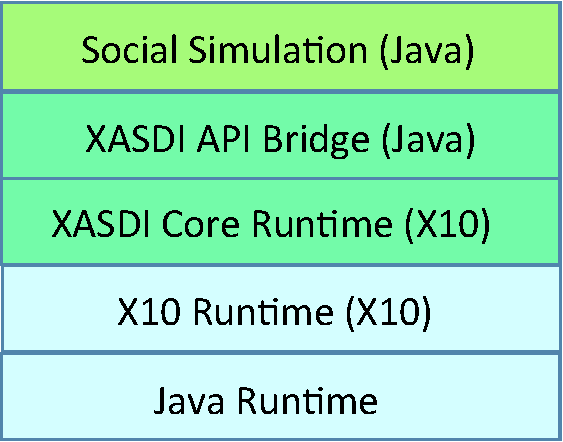
\includegraphics[width=4cm]{Figs.mizuta/xasdistack.pdf}
  \caption{XASDI Software Stack}
  \label{fig:Figs.mizuta/xasdistack}
\end{figure}


The agent in XASDI is referred to as Citizen and Citizen has corresponding CitizenProxy that is managed in the simulation environment to exchange messages.
To manage CitizenProxy, XASDI provides a hierarchical container structure called Place, Region and World (see Figure~\ref{fig:Figs.mizuta/xasdiclass}. CitizenProxies belong to a Place and Places belong to a Region. World can contain several Regions, but usually there is only one Region in the World.


Here, we need to note that the confusing terminology of the X10 programming language and the framework.
The X10 use the term ``Place'', too, but the meaning of the term is different.
The Place of X10 is used to denote the distributed execution environment for multi-core or multi-node.
For this meaning, we will use ``X10 Place (node)'' in distinction from the Place container of agents.
Only one World instance exists in one X10 Place and manages lists of entities in the world including Region and Citizen.
The world can also contain IDs of Citizens in other nodes.

\begin{figure}[h]
  \centering
  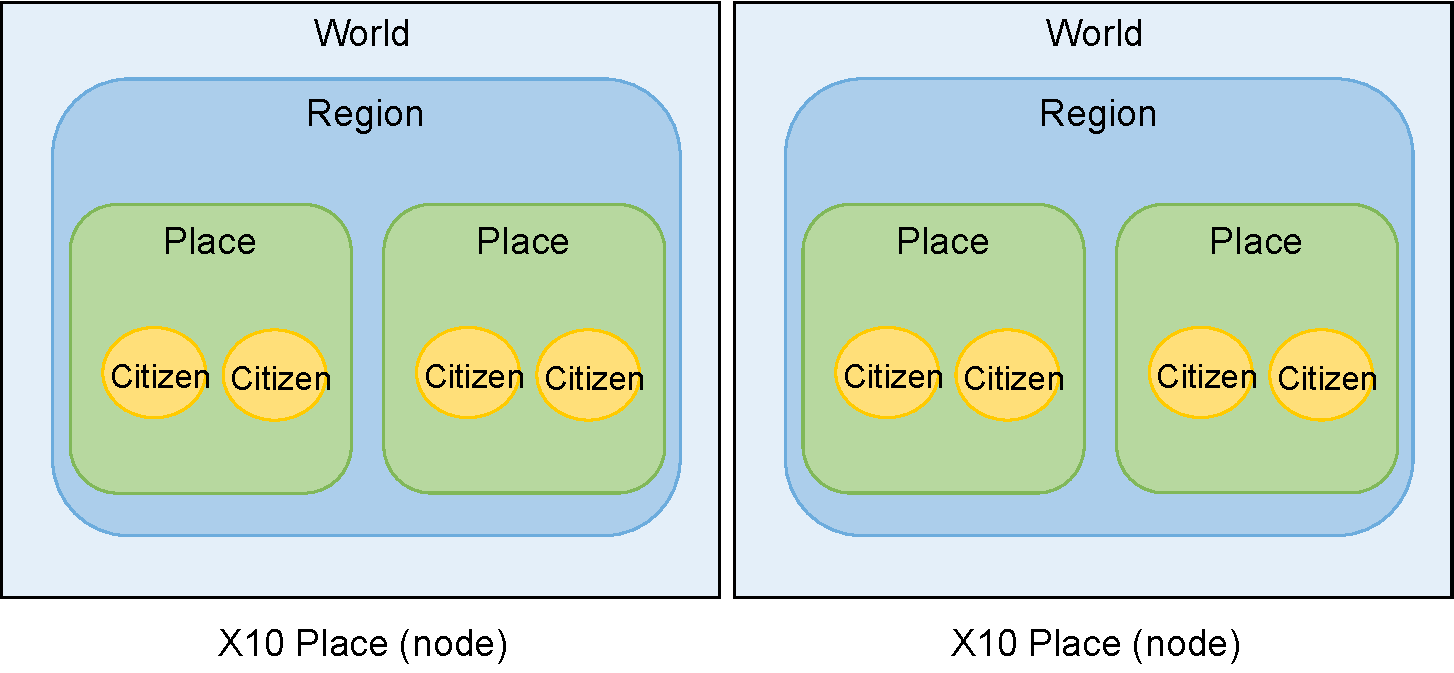
\includegraphics[width=8cm]{Figs.mizuta/xasdiclass.pdf}
  \caption{XASDI hierarchical structure to manage agents}
  \label{fig:Figs.mizuta/xasdiclass}
\end{figure}

Other important classes in XASDI are Message, MessageRepository and Driver.
MessageRepository manages Message exchange among CitizenProxy and environment and this class also works as interface between Java environment and X10 environment to exchange Messages in distributed X10 Places.
Driver manages execution of the simulation with a corresponding thread. Each Driver is related to Places (and Citizens in the Places) where it has a responsibility for execution.

Finally, XASDI provides a logging mechanism. By preparing log definitions for the application, it can output the simulation log at each X10 Places. 


Application users of XASDI need to develop their own simulation application by utilizing these classes and execute the application with XASDI library on Java and X10.
We describe the execution process on XASDI and the simple customization for the sample application bundled with XASDI.

A user starts the simulation by executing the shell script to invoke the X10 core runtime.
After the preparation of X10 environment, Launcher for the simulation written by Java is called at each X10 Place.
Launcher reads the initialization file and generates a Region, Places and Drivers.
If agents are needed to exist from the beginning of the simulation, Launcher or Driver generates Citizens.
Citizens can also be generated by Driver through the method of the Region during the simulation at given time or randomly. For example, consumer agents are generated when they enter a shopping mall.

The main simulation process is executed through Drivers.
Simulation managers in the X10 core environment generate threads and invokes call back method in each Driver in parallel.
One simulation time step can be divided into phases. The number of phases are determined at the beginning of the simulation with initialization file.
The method of the Driver looks at the time and phase given by the environment and determines the action that the corresponding Places and Citizens should perform.


In one node, there is one Region instance that manages the execution of the simulator.
The core framework written using X10 manages the Regions and Message Repositories of distributed nodes.
The Message Repository supports several kinds of messages such as individual message, broadcast message, and control message to move agent between X10 Places.
An individual message is a standard message from one agent to another.
A broadcast message is sent to all nodes and received by the Region or agents corresponding to the type of message.
A move message is a control message for X10 core runtime to remove the Citizen at the source node and restore it at the destination node with serialized field data stored in the message.


As applications for large-scale simulation on XASDI, we developped a large-scale traffic simulator for city~\cite{osogami2013toward} and a shopping mall simulator with integrated model of walking and purchasing behavior~\cite{mizuta2017wsc}.
Fig.~\ref{fig:Figs.mizuta/xasdiscaling} shows the weak scaling performance of XASDI by using our application for shopping mall simulation with distributed consumer agents~\cite{ppl2018takeuchi}.
\begin{figure}[h]
  \centering
  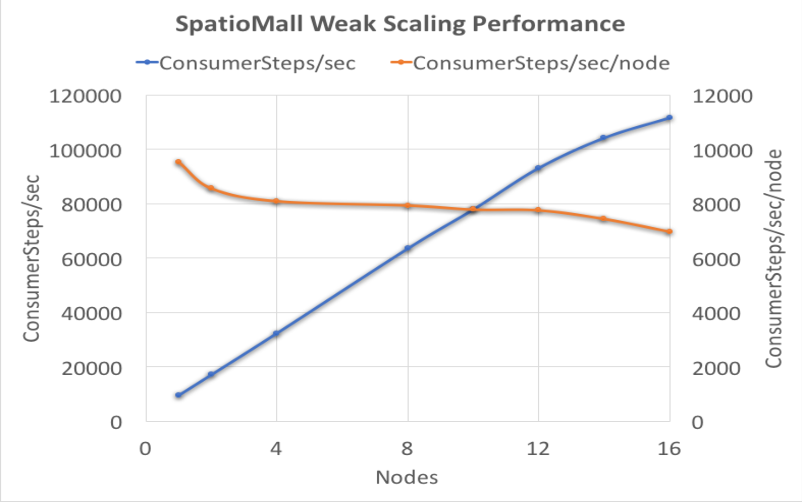
\includegraphics[width=8cm]{Figs.mizuta/xasdiscaling.pdf}
  \caption{Weal scaling performance of XASDI with shopping mall application.}
  \label{fig:Figs.mizuta/xasdiscaling}
\end{figure}




%%----------------------------------------------------------------------
\section{Applications}
\label{s:Applications}
%% - - - - - - - - - - - - - - - - - - - - - - - - - - - - - - - - - - -

%%--------------------------------------------------
\subsection{Market Simulation}
\label{ss:Market Simulation}
%% - - - - - - - - - - - - - - - - - - - - - - - - -
(Izumi)

%%++++++++++++++++++++++++++++++++++++++++++++++++++++++++++++++++++++++
\begin{figure}
  \centering
  \includegraphics[width=.8\linewidth]{Figs.noda/figure-07.market_phase.eps}
  \caption{Phase Diagram of Market Simulation}
  \label{fig:Figs.noda/figure-07.market_phase.eps}
\end{figure}
%%++++++++++++++++++++++++++++++++++++++++++++++++++++++++++++++++++++++



%%--------------------------------------------------
\subsection{Pedestrian Simulation}
\label{ss:Pedestrian Simulation}
%% - - - - - - - - - - - - - - - - - - - - - - - - -
CASSIA Framework can illustrate a trade-off structure of social problems.
The most of social problems like planning of evacuations from disasters
are not simple optimization problems but dilemmas among multiple
objective functions.
We will show an example to apply CASSIA Framework to find
such trade-off structures using evacuation planning for Nishiyogogawa-ku, Osaka,
which includes over 300 control parameters\cite{Noda2018b}.
Because of the large degrees of freedom,
the search space of this problem is so huge
that the solution of this problem require high-performance
computing like K-computers.


%%------------------------------
\subsubsection{Pedestrian simulator: CrowdWalk}
\label{sss:CrowdWalk}
%% - - - - - - - - - - - - - - -
In order to simulate evacuation situations, we employ CrowdWalk
\cite{yamashita:2013,yamashita:2014a}.
CrowdWalk is a pedestrian simulator that limits human movement 
to one-dimensional movement on the road network. 
Road network is composed of nodes and links,
on which CrowdWalk controls 
large number of pedestrian movements at high speed.

We use a road map of Nishiyodogawa-ku,
which consists of 7,624 nodes (intersections) and 10,707 road links
(\figref{fig:Figs.noda/figure-08.nishiyodogawa.eps}).
This area has 86 official refuges
and 54,909 of the population,
which are distributed in 146 small zones.
We suppose that every people in each zone follows one guidance rule
that requests them to go to a certain destination with one via point in a map.
The destination and the via point are selected from the 86 official refuges
and from 533 major intersections, respectively.

%%++++++++++++++++++++++++++++++++++++++++++++++++++++++++++++++++++++++
\begin{figure}
  \centering
  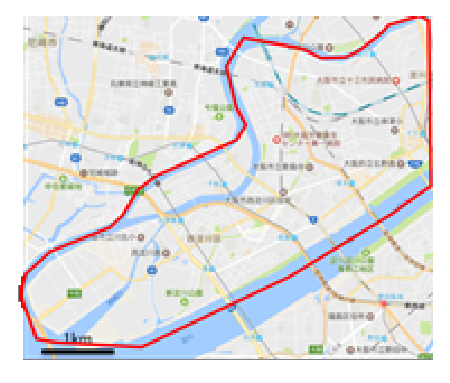
\includegraphics[width=.49\linewidth]{Figs.noda/figure-08.nishiyodogawa.eps}~
  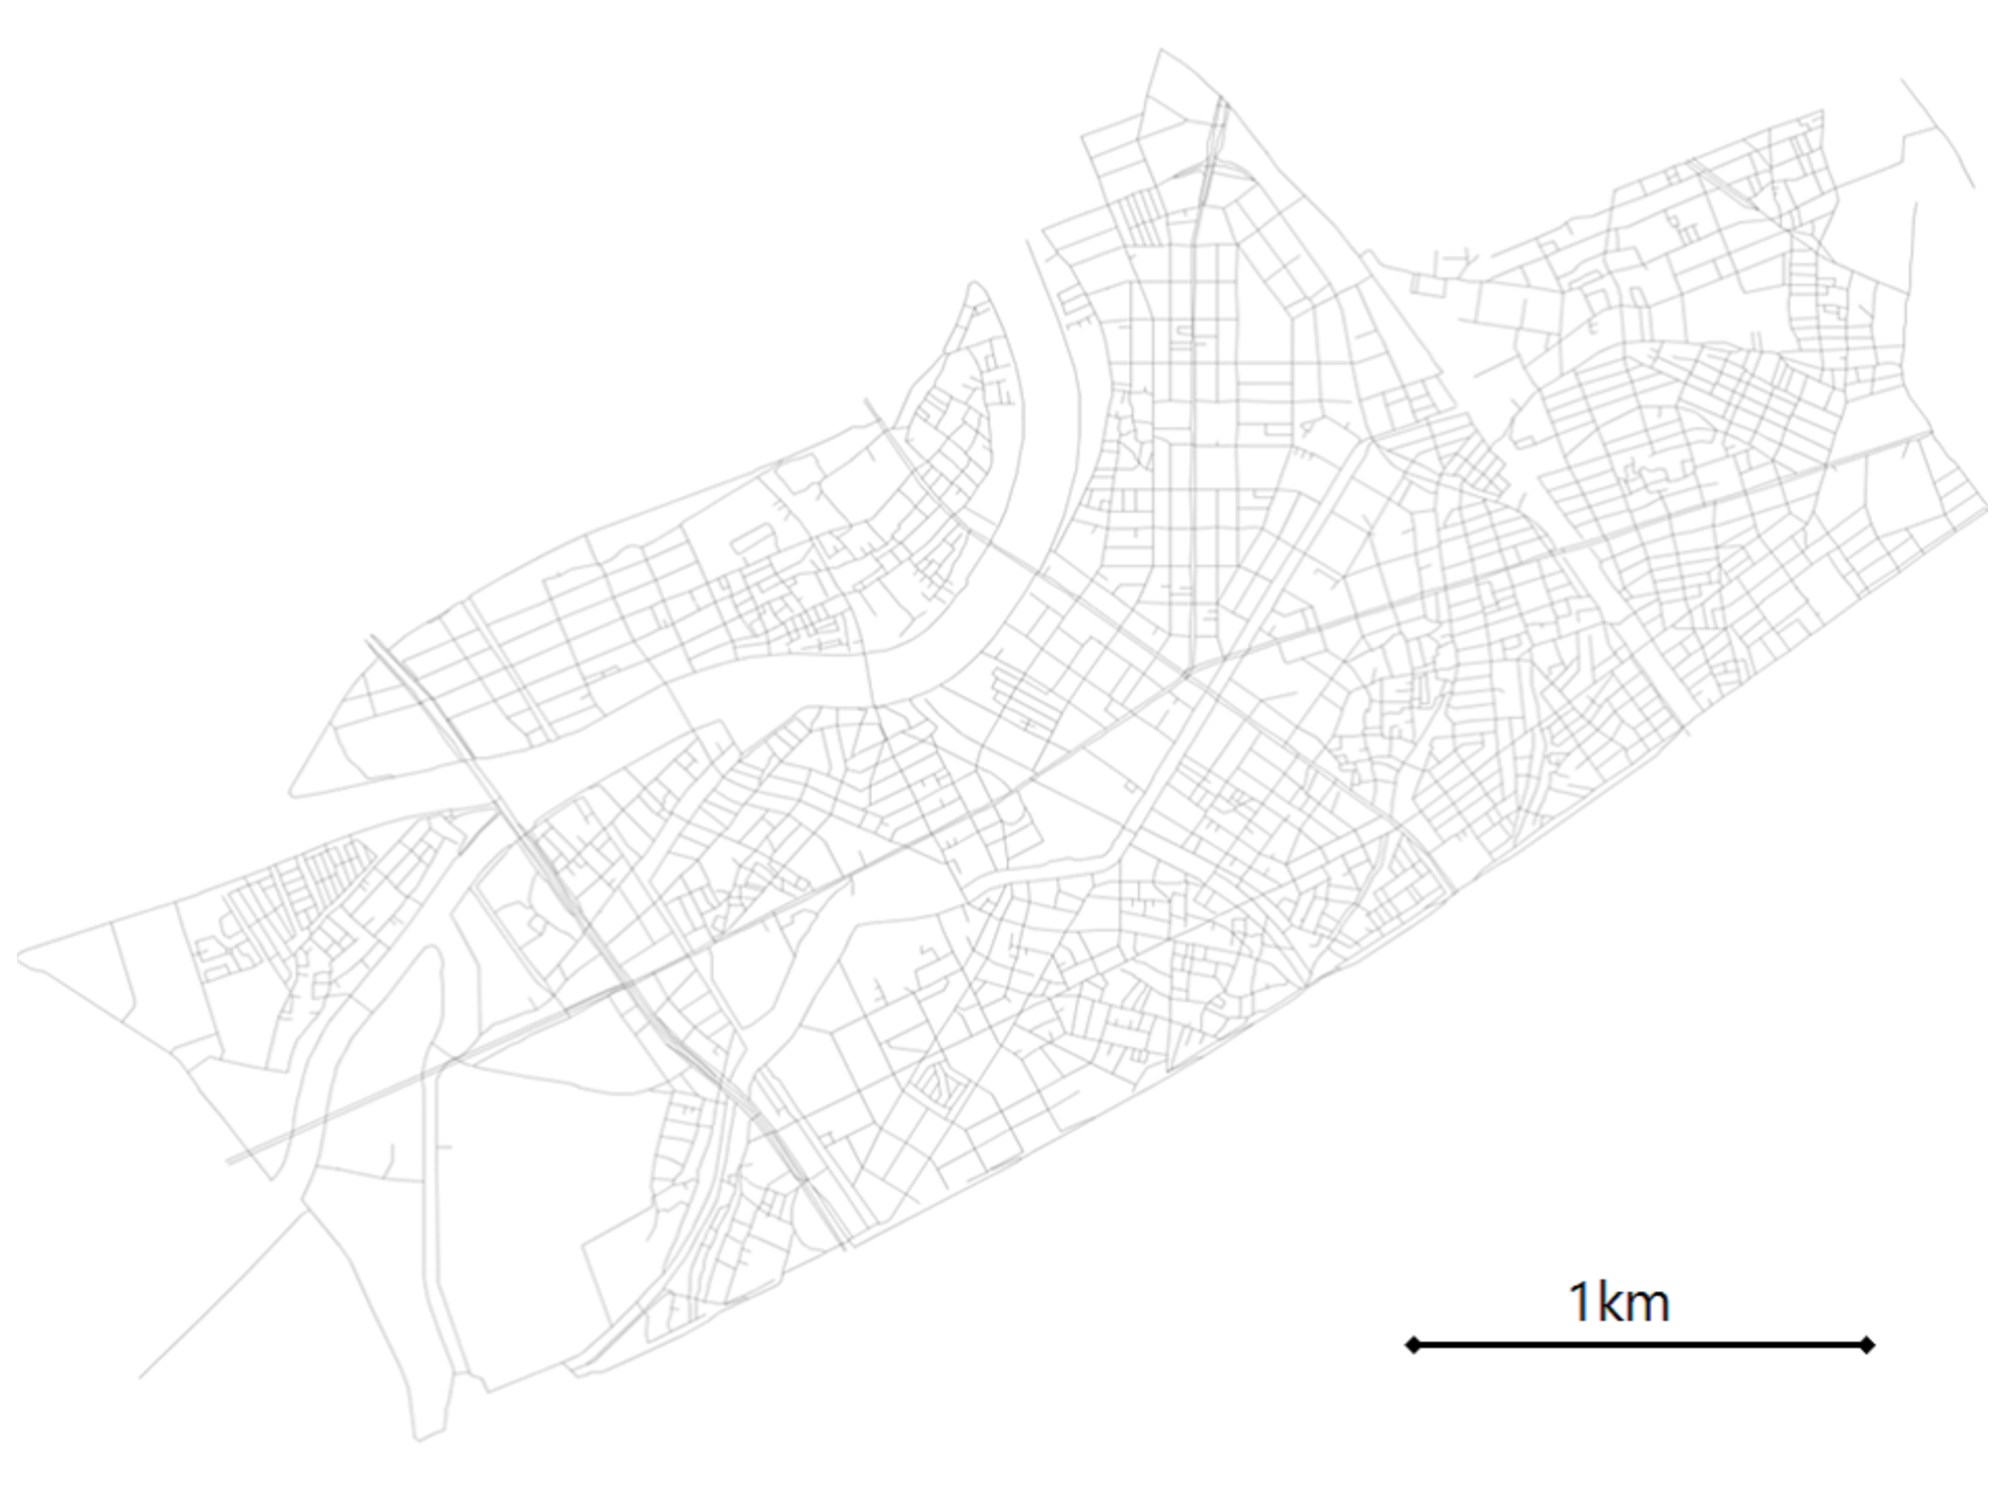
\includegraphics[width=0.49\linewidth]{Figs.noda/yodogawa_map}
  \caption{Nishiyodogawa Area (left) and
    Road Map (right) used in Pedestrian Simulation}
  \label{fig:Figs.noda/figure-08.nishiyodogawa.eps}
\end{figure}
%%++++++++++++++++++++++++++++++++++++++++++++++++++++++++++++++++++++++

%%------------------------------
\subsubsection{Multi-Objective Optimization}
\label{sss:moea}
%% - - - - - - - - - - - - - - -

in general, evacuation planning includes a dilemma
between evacuation time and simple-ness of evacuation guidance.
From the viewpoint of the minimization of evacuation time,
it is better to use the result of mathematical optimization
like maximum network-flow \cite{kobayashi:2016}.
However, we need to guide large number of people that include
persons who are not acquainted with the place like visitors.
So, the guidance should be simple enough to understand and to follow easily.


In order to know the relationship of these two objectives,
we apply NSGA-II(Elitist Non-Dominated Sorting Genetic Algorithm)
\cite{deb:nsga}, a genetic algorithm for
multiple objective optimization.

For the first objection function, the evacuation time,
is estimated by simulation using CrowdWalk for each guidance plan.

For the second objective function, the simple-ness of evacuation guidance,
we introduce `entropy' of the plan as follows.
Suppose two connecting zones, $z_i$ and $z_j$ in the area,
whose populations are $n_i$ and $n_j$, respectively.
If the two rules for these zones has same via point and destination,
then the entropy is zero.
Otherwise, 
the entropy of this pair is defined by:
\begin{eqnarray}
  H(z_i,z_j) & = & - (n_i/(n_i + n_j))\log(n_i/(n_i + n_j))
                  - (n_j/(n_i + n_j))\log(n_j/(n_i + n_j))
                  .
                  \nonumber
\end{eqnarray}
Finally, we use total entropy $H = \sum_{z_i,z_j} H(z_i, z_j)$
for the index of the complexity of the guidance (opposite value
of the simple-ness).


% %%++++++++++++++++++++++++++++++++++++++++++++++++++++++++++++++++++++++
% \begin{figure}
%   \centering
%   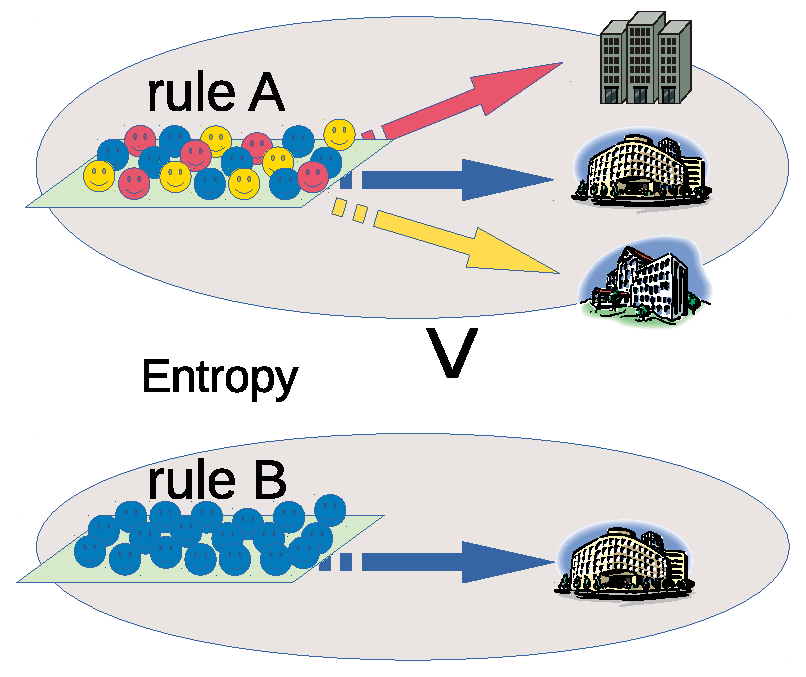
\includegraphics[width=.5\linewidth]{Figs.noda/figure-09.evac_rule.eps}
%   \caption{Rule Entropy}
%   \label{fig:Figs.noda/figure-09.evac_rule.eps}
% \end{figure}
% %%++++++++++++++++++++++++++++++++++++++++++++++++++++++++++++++++++++++

%%------------------------------
\subsubsection{Experimental and Discussion}
\label{sss:nsga-experiment}
%% - - - - - - - - - - - - - - -

In order to run NSGA-II for this guidance plan,
we utilized OACIS described in \secref{ss:OACIS} to manage the large number of runs.
The search space of this problem is so huge
($R^{73} \times 533^{146} \times 86^{146}$)
and NSGA-II requires large number of populations (about 100--1,000).
So we need to run so many runs for the optimization.
In the experiment, we runs 500 generations with 100 population
for the optimization,
which means we run 500,000 simulations
\footnote{We runs 10 simulations for one guidance plan
  to calculate average evacuation time.}
for this experiment.

To control 
We implemented NSGA-II procedure using Ruby API of OACIS.
In the actual GA procedure, we use `simulated binary crossover' and
`polynomial mutation' for creating new generations,
and Paleto ranking mechanism to determine the selection.


\Figref{fig:Figs.noda/figure-11.evac_wide.eps} shows the result
of the experiment.
In this graph, vertical and horizontal axes indicate
evacuation time and the complexity of plan (total entropy
scaled by 100), respectively.
The color of the dot indicates the generations.
From this result,
we can see that the evacuation plans are improved by progress
of generations, and almost saturate to boundary of 3000 for
evacuation time and 2100 for complexity of guidance.
In order to minimize the evacuation time,
we need to choose relatively complex guidance (the complexity is about 2200
rather than 2100).
On the other hand, if we consider simplify the complexity,
the evacuation time increase drastically up to 7000.
And, we can see reasonable guidance will exist the most left-bottom
area of the Paleto front in this graph.

%%++++++++++++++++++++++++++++++++++++++++++++++++++++++++++++++++++++++
\begin{figure}
  \begin{minipage}[c]{.49\linewidth}  %{width}
  \centering
  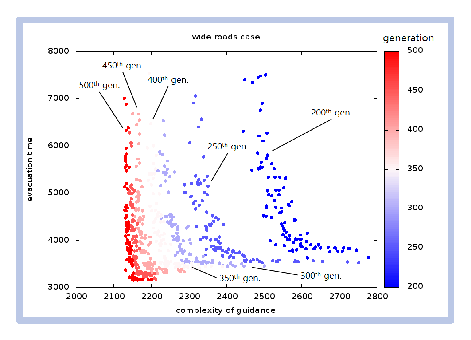
\includegraphics[width=.99\linewidth]{Figs.noda/figure-11.evac_wide.eps}
  \caption{Result of Evacuation Simulation (wide road)}
  \label{fig:Figs.noda/figure-11.evac_wide.eps}
  \end{minipage}~
%\end{figure}
%%++++++++++++++++++++++++++++++++++++++++++++++++++++++++++++++++++++++
%%++++++++++++++++++++++++++++++++++++++++++++++++++++++++++++++++++++++
%\begin{figure}
  \begin{minipage}[c]{.49\linewidth}  %{width}
  \centering
  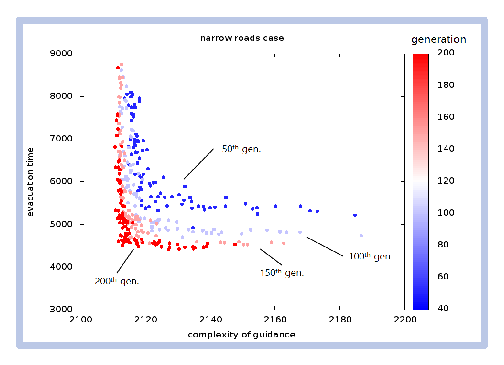
\includegraphics[width=.99\linewidth]{Figs.noda/figure-10.evac_narrow.eps}
  \caption{Result of Evacuation Simulation (narrow road)}
  \label{fig:Figs.noda/figure-10.evac_narrow.eps}
  \end{minipage}
\end{figure}
%%++++++++++++++++++++++++++++++++++++++++++++++++++++++++++++++++++++++


\Figref{fig:Figs.noda/figure-10.evac_narrow.eps} also
shows the result of the case that the people use only pedestrian road.
In this case, the boundary of the evacuation time increase to 4500,
but the complexity of guidance is similar to the previous case.
Anyway, in both cases of \figref{fig:Figs.noda/figure-11.evac_wide.eps} and
\ref{fig:Figs.noda/figure-10.evac_narrow.eps},
we can see a clear trade-off structure of Paleto solution sets.

This result imply that
OACIS with evolutionary methods have a great potential
to investigate such social problems.
We also succeed to apply CARAVAN to run the same procedure
on K-computer.
This combination enables to run larger scale of simulations
and search spaces.




%%--------------------------------------------------
\subsection{Traffic Simulation}
\label{ss:Traffic Simulation}
%% - - - - - - - - - - - - - - - - - - - - - - - - -
%(Hattori, Ito?)

%%--------------------------------------------------
%\subsection{Traffic Simulation}
%\label{ss:Traffic Simulation}
%% - - - - - - - - - - - - - - - - - - - - - - - - -
%(Hattori, Ito?)

% Car traffic is one of popular targets of social simulations, and it is applied to various objectives, for example, traffic control, city design, economic activities, and 
% environmental issues. In this CASSIA project, some traffic simulations and their analyses have been achieved not only in applications and also in basic modelings, applying and assuming 
% present and future supercomputers. 

%%------------------------------
\subsubsection{Simulation cost and benchmark}
%% - - - - - - - - - - - - - - -

Traffic simulations are comprised of three parts: road map with traffic rules and regulations, 
origin and destination(OD) sets of cars with travel routes, and movements of cars on the map 
along their routes. 
There are two method to parallelize traffic simulations. One is to parallelize geometrically, and the other car- or trip-wisely. 
Geometrical parallelization is advantageous on modern supercomputers, because necessary data transfer is states of cars which move out from an area on one node and go to an area on other node, 
and only nearest-neighbor communications appear. 

Parallelization of trip routings is more complicated but most trips are short range and are executed on one node using local map. 
Time comsuming long trips are few, and their routing cost can be made negligible. 

% Simulation of car movements can be made very simple and also very complicated. In case of normal traffic without hazardous conditions like accidents or disasters, 
% it is sufficient to execute few arithmetic operations per car using distance to a car in front and legal speed limit, which determe appropriate velocity that the car does not crash to 
% a car in front and does not break the legal limit. 
% To the contrary, heavy operations are necessary to simulate high-resolution movements of car to study, for example, risk of traffic accidents and weather effects. 
% Hydrodynamic and/or machine engineering simulations solving PDE with high reliability in space and time will be executed. In this extreme, simulations of just one car may require 
% Exa-scale computers. 

Parallelization feature of car traffic simulations with the most parallelization demanding case, that is, simulations using the simplest car movement was measures in this CASSIA project. 
Each car continues to move along road, and turn randomly at each crossing. This means that no routing is done. This simulation model will require the lightest processing 
in each computer node, and the most frequent  inter-node communication. 
Results of strong scaling of parallelized performance using the K computer up to its quarter configuration(20,736 nodes) for the traffic simulation on entire road of Japan are shown
 in \figref{itoallJapan}. 
Simulations were up to 100 second and time step was 0.01 second. So totally 10,000 steps were done for about 11.7 million cars on totally 1.28 million kilometer-long  roads 
using the ``Open Street Map''. Using the quarter nodes, simulations of 10,000 steps were executed in 11.5 second apart from the initial preparation(66.1 second), 
and efficient parallelization is confirmed. 
For another simulation of 100 million car on all-over the world with 30.9 million kilometer took 116 second using quarter nodes of the K computer. 

This result implies that realtime or faster car-traffic simulation will be executed on the K and the future supercomputers. 

\begin{figure}
 \begin{minipage}[c]{.49\linewidth}  %{width}
 \centering
  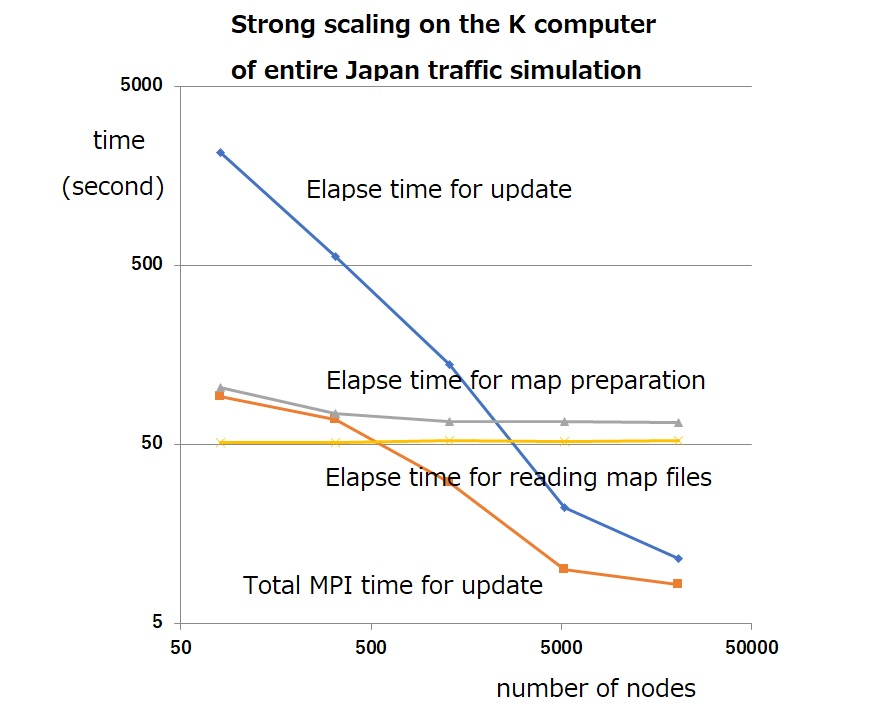
\includegraphics[width=0.99\linewidth]{Figs.ito/allJapan.jpg}
  \caption{Results of strong scaling using the K computer for entire Japan traffic simulation with the simplest movements without routings are plotted.   }
  \label{itoallJapan}
 \end{minipage}~
 \begin{minipage}[c]{.49\linewidth}  %{width}
 \centering
  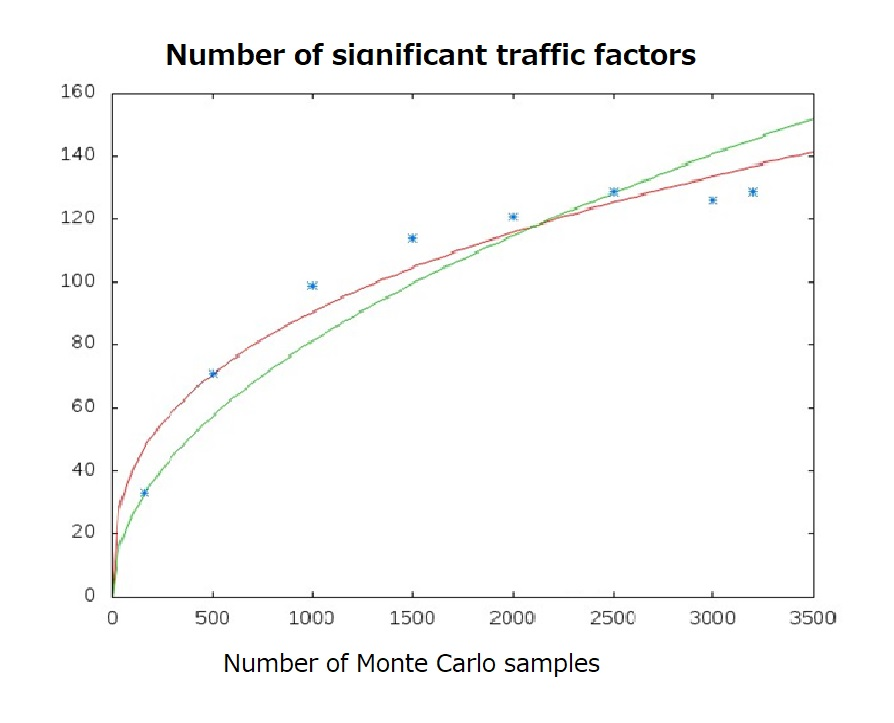
\includegraphics[width=.5\linewidth]{Figs.ito/Factors.jpg}
  \caption{Number of factors estimated using a factor analysis are plotted. Green curve shows square root of number of Monte Carlo samples, which is expected in the case of uniform 
distribution of eigenvalues of correlation matrix, but this plot is interpolated by slower red curve. }
  \label{itoFactor}
 \end{minipage}
\end{figure}


%%------------------------------
\subsubsection{Traffic factors}
%% - - - - - - - - - - - - - - -

In traffic simulation models, numbers of input parameters and output results are enormous. Each car has several input parameters, for example, its origin, destination, 
starting time, driving preference and also several output parameters, for example, travel duration and gas consumption. 
Each traffic signal has its control parameters. Each road segment has its speed limit and car flux. 
Such parameter-number explosion is quite common in various social models. 
In Kobe city, as an example, there are more than 30,000 road segments and about 100,000 trips(OD pairs) daily. So the number of input parameters 
and output results are order of $10^5$ at least. 
Without knowing behavior of simulation model, we cannot apply the model to describe, predict and design the real phenomena. 
But it is impossible to tame a model with $10^5$ input and output. 
So the first step is to eliminate unimportant parameters and to extract relevant parameters. 
A standard method for this purpose is the multivariate statistical analysis. 

In this CASSIA project, a car-traffic model and simulator of Kobe city was developed \cite{Ito1}. Using this simulator, Monte Carlo simulations for various OD sets satisfying a constraint 
that daily trips be 100,000 and 70\% of the trips are coming from peripheral cities and just passing through Kobe city. A factor analysis was applied to the output flux of road segments\cite{Ito2}.  
Numbers of estimated factors are plotted in \figref{itoFactor}. It is observed in this \figref{itoFactor} that thousands of samples finally clarifies hundreds of factors. 
Hundreds are still large, but anyway we succeeded to extract relevant factors. 

This is still a model analysis, but this result will suggest that we will need to measure traffic thousands times to extract the relevant factors from real traffic phenomena, 
but real traffic will never repeat the same traffic thousands times. So we can use plausible computer simulation models to get better description of the real social phenomena. 

% \noindent {\bf References}
% 
% \noindent [Ito1]Yuta Asano, Nobuyasu Ito, Hajime Inaoka, Tetsuo Imai and Takeshi Uchinane, Proceedings of the International Conference on Social Modeling and Simulation, plus Econophysics Colloquium 2014(Springer Proceedings in Complexity, ISBN 978-3-319-20590-8), p. 255-264, 
% {\it Traffic Simulation of Kobe-City}. 
% 
% \noindent [Ito2]Takeshi Uchitane and Nobuyasu Ito, "Applying Factor Analysis to Describe Urban Scale Vehicfle Traffic Simulation Results," (in Japanese) 
% Journal of the Society of Instrument and Control Engineers vol.52 (2016) No.10 p.545-554. 
% 
% %[Ito1] Hideyuki Mizuta, Takashi Imamichi, �gLarge-scale social simulation framework "X10-based Agent Simulation on Distributed Infrastructure (XASDI)�h and applications�h, AROB 23nd 2018 , B-Con PLAZA, Beppu. JAPAN ,Jan. 19, 2018.
% 

%%--------------------------------------------------
\subsection{Traffic Simulation}
\label{ss:Traffic Simulation}
%% - - - - - - - - - - - - - - - - - - - - - - - - -
(Hattori, Ito?)

Real-life urban traffic flows consists of different types of vehicles, each of which has its own properties of behaviors. In the project, taxi is our primary target. 

\paragraph{Behavior Analysis of Taxi Drivers and Model Construction}
We use probe-car data provided by a taxi company in Kyoto city for a one month period including approximately 700,000 location data points recorded per day.
%
In general, the driver’s behavior in VACANT state is driver-determined. That is, after dropping off passenger(s), a driver can freely select next destination and mode (queuing or cruising) for picking up the next passenger(s). In contrast, the destination in OCCUPIED state is passenger-determined. Given this fact, we hypothesize that the tendency of the location that a taxi driver got passenger(s) would be one of the main characteristics of the driver. For considering that, we focused on the preferred location to pick up passenger(s) and try to classified drivers based on that. 

\begin{figure}
  \centering
  \includegraphics[width=.9\linewidth]{Figs.hatto/fig-hatto-01.eps}
  \caption{Visualization of Origins for each Cluster : Red (High Ratio)⇔ Blue (Low Ratio)}
  \label{fig:Figs.hatto/fig-hatto-01.eps}
\end{figure}

To extract popular regions to get passenger(s), we apply kernel density analysis and the mean shift clustering algorithm which are widely used for extracting POI (Point of Interest) from the two-dimensional information provided by photo geo-tagging and GPS \cite{Crandall06a}. From the results of Kernel density analysis, we can assume that the activity range defining the average driver’s interest point is 50 seconds of longitude and latitude.  We use these values as the bandwidth for the Mean-Shift clustering algorithm so that we got 15 regions. We then calculated the ratio of picking up passenger(s) at each region. We use the ratios and the affinity propagation clustering algorithm to classify all taxi drivers. This yielded 10 clusters of driver type.
Figure 1 shows the departure points for the clusters. These figures clearly indicate drivers tend to favor a specific territory for picking up passenger(s) . For example, 112 drivers for Cluster 1 tend to operate on the north side of Kyoto City. On the other hand, 33 drivers Cluster 4 are apt to go to the south side. 

\begin{figure}
  \centering
  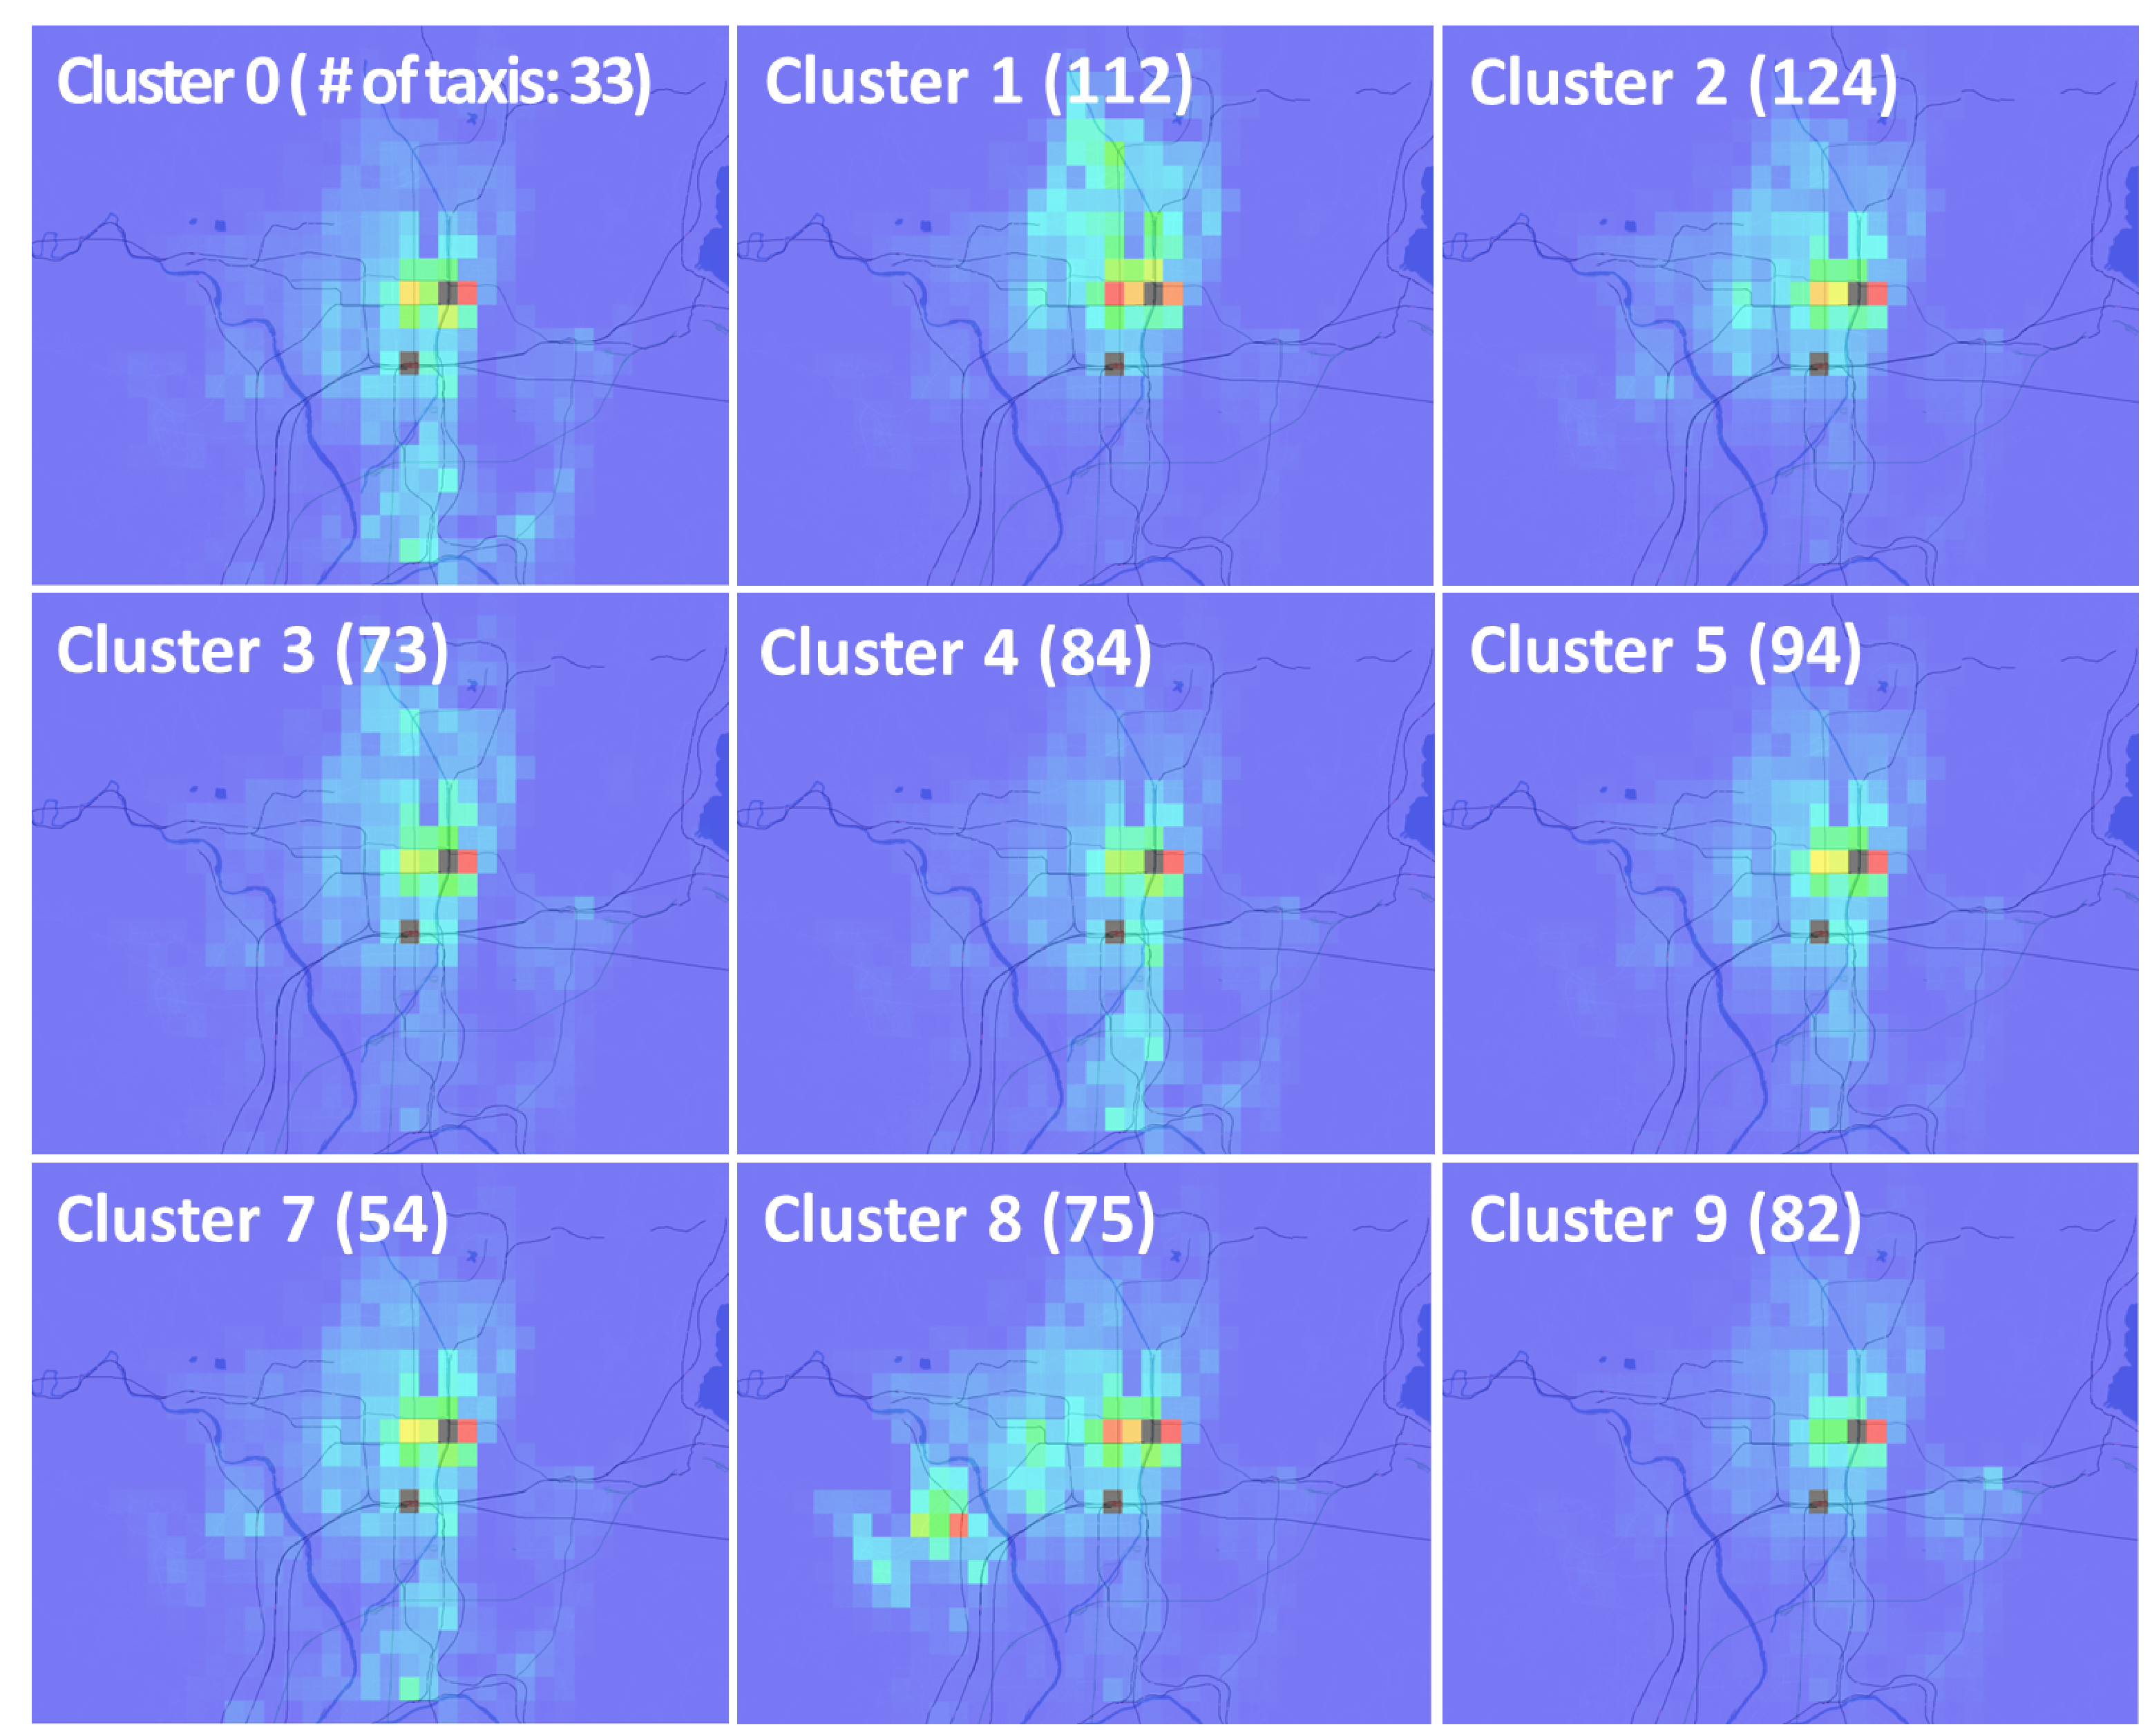
\includegraphics[width=.7\linewidth]{Figs.hatto/fig-hatto-02.eps}
  \caption{Comparison of Characteristic Behavior Model and Uniform Model}
  \label{fig:Figs.hatto/fig-hatto-02.eps}
\end{figure}

\begin{table}[]
\centering
\caption{Ratio of Staying Time in each Region}
\label{tbl:ratio-of-staying}
\begin{tabular}{|c|c|c|c|c|}
        \hline
        & \multicolumn{2}{|l|}{Probe-Data} & \multicolumn{2}{|l|}{Behavior Model} \\
        \hline
        & Cluster1       & Cluster4      & Cluster1         & Cluster4        \\
        \hline
Region3 & 0.263          & 0.056         & 0.217            & 0.095           \\
        \hline
Region4 & 0.016          & 0.196         & 0.054            & 0.165          \\
        \hline
\end{tabular}
\end{table}

In simulations each taxi agent has two states: OCCUPIED and VACANT. When the state changes from OCCUPIED to VACANT, taxi agents stochastically decide next destination and mode according to current time zone and current location. To analyze this decision-making process, we construct 10 driver models based on the clustering results shown in Figure 1. Further, if the taxi picks up a passenger(s) and changes their state to OCCUPIED, the destination is given by the passenger agent. Each passenger agent has an OD matrix whose contents stochastically mirror the probe-car data. In this taxi model, the driver type is given by 1) ratio of Queuing/Cruising, and 2) selection of area used in searching for passenger(s).
We conduct traffic simulations in the City of Kyoto with constructed taxi agents.
Figure 2 shows a visualization of agents whose model followed taxi driver cluster ID 1 or ID 4. ID 1 is a driver who tends to work in the northern part of Kyoto City while ID 4 is in the south. The characteristic behavior model confirmed that there is a deviation in the preferred areas for each taxi driver class as expected, see Figures 2(a) and (b). Table 1 lists the ratios of staying time in each region. Comparing probe-car data, it seems that the tendencies of agents follow the clustering result.







%%----------------------------------------------------------------------
\section{Computational Roadmaps of Social Simulations and Future}
\label{sec:Computational Roadmaps of Social Simulations}
%% - - - - - - - - - - - - - - - - - - - - - - - - - - - - - - - - - - -

In this project, we also try 
to determine how HPC contributes
to the advancement of research on social simulation or
to clarify the computational power required
for real applications of social simulation.
In this section, we focus on three applications and try
to develop roadmaps for them
\cite{Noda2018a}.

In the development of these roadmaps, 
we adopted two indexes to measure the computational cost,
``number of situations'' and ``complexity of one simulation session''.
We considered exhaustive evaluation by simulation as 
a key methodology of social simulation.
Therefore, to evaluate the model,
examining many conditions and models is important.
The index of ``number of situations'' indicates this number.
Meanwhile,
ordinal computational cost of a simulation,
which is determined by the number of entities and the number
of interactions among the entities,
is important.
In addition, in multiagent simulation,
the computational cost of thinking of each agent is significant.
In the following discussion, we integrate these complexities
as ``complexity of one simulation session''.

%%--------------------------------------------------
\subsection{Evacuation/Pedestrian Simulation}
%% - - - - - - - - - - - - - - - - - - - - - - - - -

The main target of evacuation simulation is not
to find an optimal plan of evacuation for a given disaster situation,
but to evaluate the feasibility and robustness of executable candidates
of evacuation plans or guidance policies.

Several simulations have been performed for 
evaluating such evacuation plans
\cite{Noda2009x}\cite{Noda2010p}\cite{Noda2010y}\cite{Yamashita2014}.
For example, a simulation of an evacuation from
a Tsunami struck city in Tokai area in Japan was performed.
We conducted the following exhaustive simulations considering various sizes and evacuation
policies (evacuee's origin-destination (OD) plans).
The simulation results tell that
the scale of evacuation can be grouped into two categories, namely,
``large'' ($>$ 3,000 evacuees) and
``small'' ($<$ 3,000 evacuees),
and that citizens and local governments should consider at least 
two plans for large- and small-scale evacuations.

We execute the evacuation simulation described above to arrive at
a reference point for illustrating computational costs of various
actual applications.
In the above simulation, we considered the following scenarios:
\begin{itemize}
  \item 2,187 OD plans and
  \item 8 cases of evacuation population (70--10,000 agents).
\end{itemize}
Therefore, in total, 17,497 simulation scenarios were executed
over about 30 days when using a single process on Xeon E5 CPU (2.7 GHz).
We denote this reference point as the rectangle
``city zone, TSUNAMI'' in \figref{fig:Figure-4}.

We can easily extend the simulation scale.
Although a population of only 10,000 is considered in ``city zone, TSUNAMI'',
we can extend the simulation to a more densely populated area such as in Tokyo.
For example,
we performed a similar simulation analysis in the Kanazawa area,
which is located on the coast along the Japan Sea and
experiences snowfall in the winter.
In this case, the population size is similar (about 6,000 agents),
but the number of combinations of scenarios increases to 4,194,304 ($2^{22}$).
The rectangle ``city zone, TSUNAMI and HEAVY SNOW'' in 
\figref{fig:Figure-4} denotes this calculation cost.

We can further extend the simulation to a large scale with a larger number of
scenarios.
Kitasenju area, a large transfer station surrounded by rivers,
has a population of 70,000, and the computational cost of simulating this area is
denoted by ``dense-population zone, complex disaster'' in \figref{fig:Figure-4}.
Because this area is densely populated and complex, 
we have combinations of 44 policy candidates,
that is $2^{44}$ scenarios.
In the case of Tokyo, we need additional computational power.
In \figref{fig:Figure-4}, ``megacity'' corresponds a huge
city such as Tokyo.  In this case, the size of evacuation and the
number of possible scenarios is very large.
Therefore, peta- or exa-scale HPC is required to handle such
simulations.

%%----------------------------------------------------------------------
\begin{figure}
  \centering
  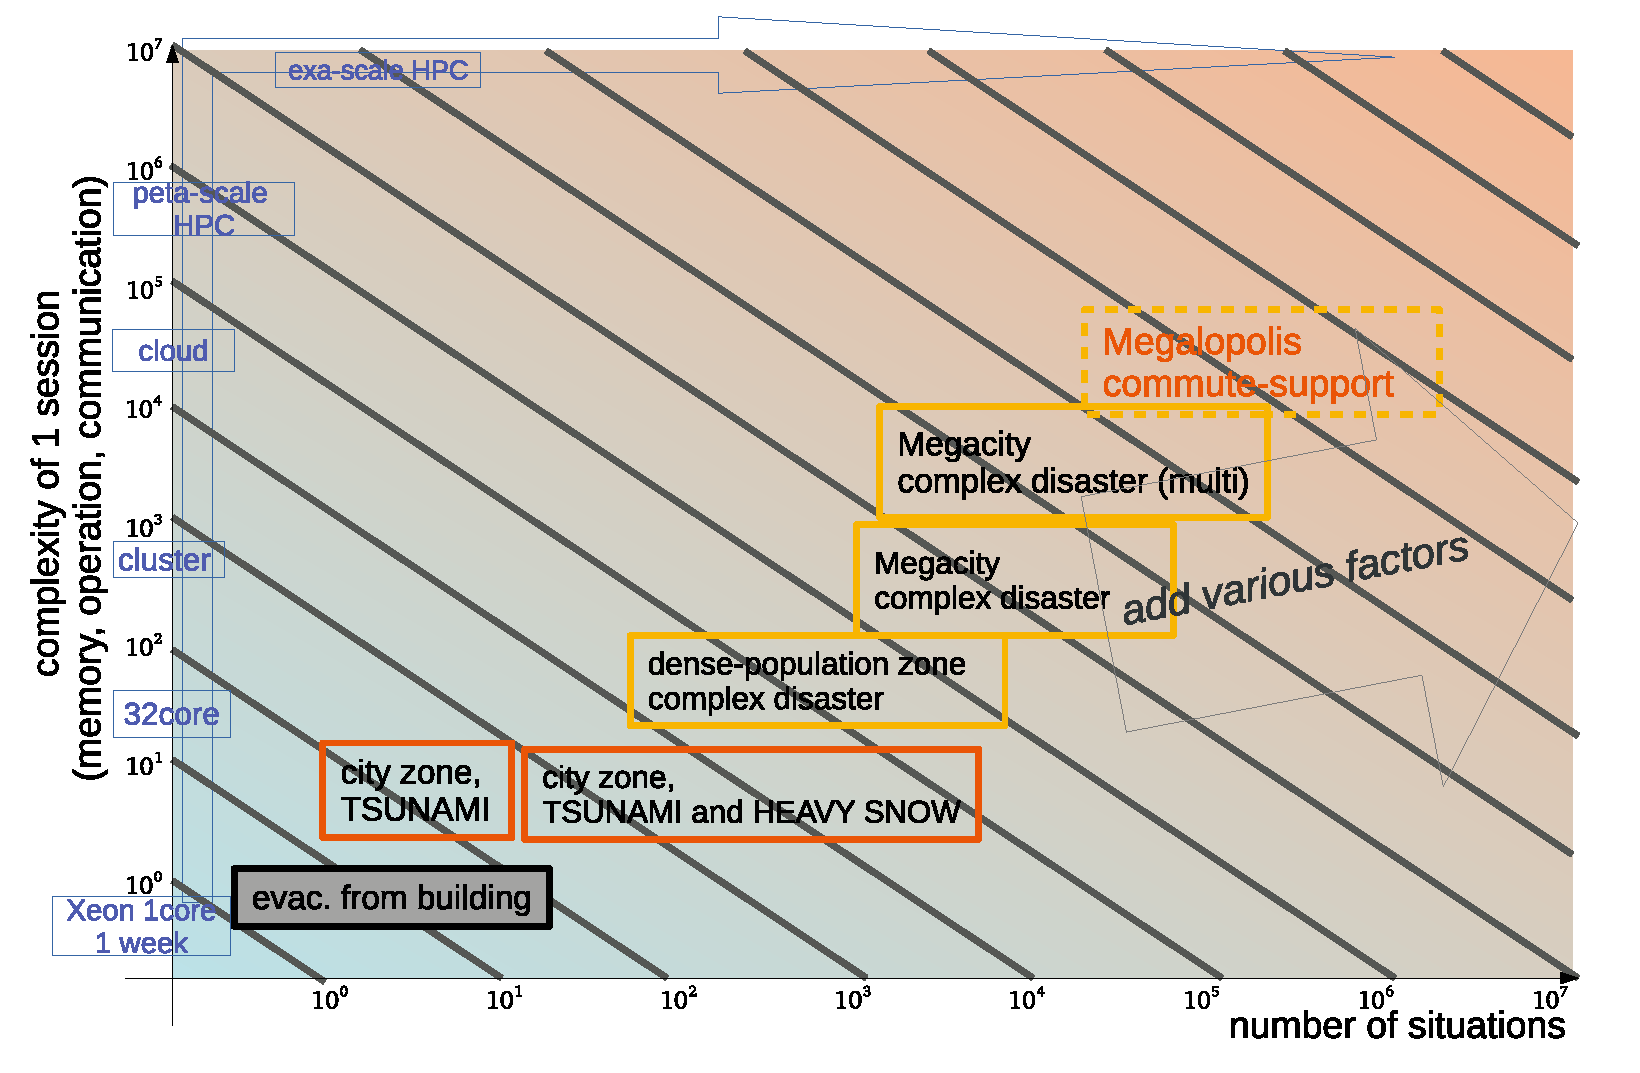
\includegraphics[width=.60\linewidth]{Figs.noda/figure2-4.eps}
  \caption{Roadmap of Evacuation Simulation}
  \label{fig:Figure-4}
\end{figure}
%%----------------------------------------------------------------------

%%--------------------------------------------------
\subsection{Traffic Simulation}
%% - - - - - - - - - - - - - - - - - - - - - - - - -

To create a reference point for the roadmap of the traffic
simulation,
we considered the case of evaluating road restriction policies
for road construction in the Hiroshima area\cite{Osogami2013b}.
In this case, we performed simulations of the following scales:
\begin{itemize}
  \item 70,000 agents (trips), 120,000 road links, and 15 hours and
  \item 20 cases
\end{itemize}
In this case, the calculation required about one day when using a single process
on Xion E5 CPU.
We denote this reference point as ``million city, road plan''
in \figref{fig:Figure-5}.

We can draw out the roadmap from this reference point.
When considering the Tokyo area,
the number of agents increases up to about 2 million
and the number of road links increases to about 610,000.
Moreover, if we consider a larger area such as the Tokyo metropolitan area,
the population increases about 4 million and the number of road links increases to 2.5 million.
These calculation costs are plotted as ``Tokyo, traffic
control'' and ``metropolis, traffic control'' in
\figref{fig:Figure-5}.

When we consider a big event,
we must list a large number of cases to evaluate the robustness
of road traffic to accidents,
whereas the scenarios mentioned above pertain to normal situations
that are repeated every day.
Because various situations affect traffics,
the number of situations increases quickly.
These costs are plotted as 
``Tokyo, big event'', ``metropolis, big event'' and ``whole Japan, big
event''
in \figref{fig:Figure-5}, and they require exa-scale computational power.


%%----------------------------------------------------------------------
\begin{figure}
  \centering
  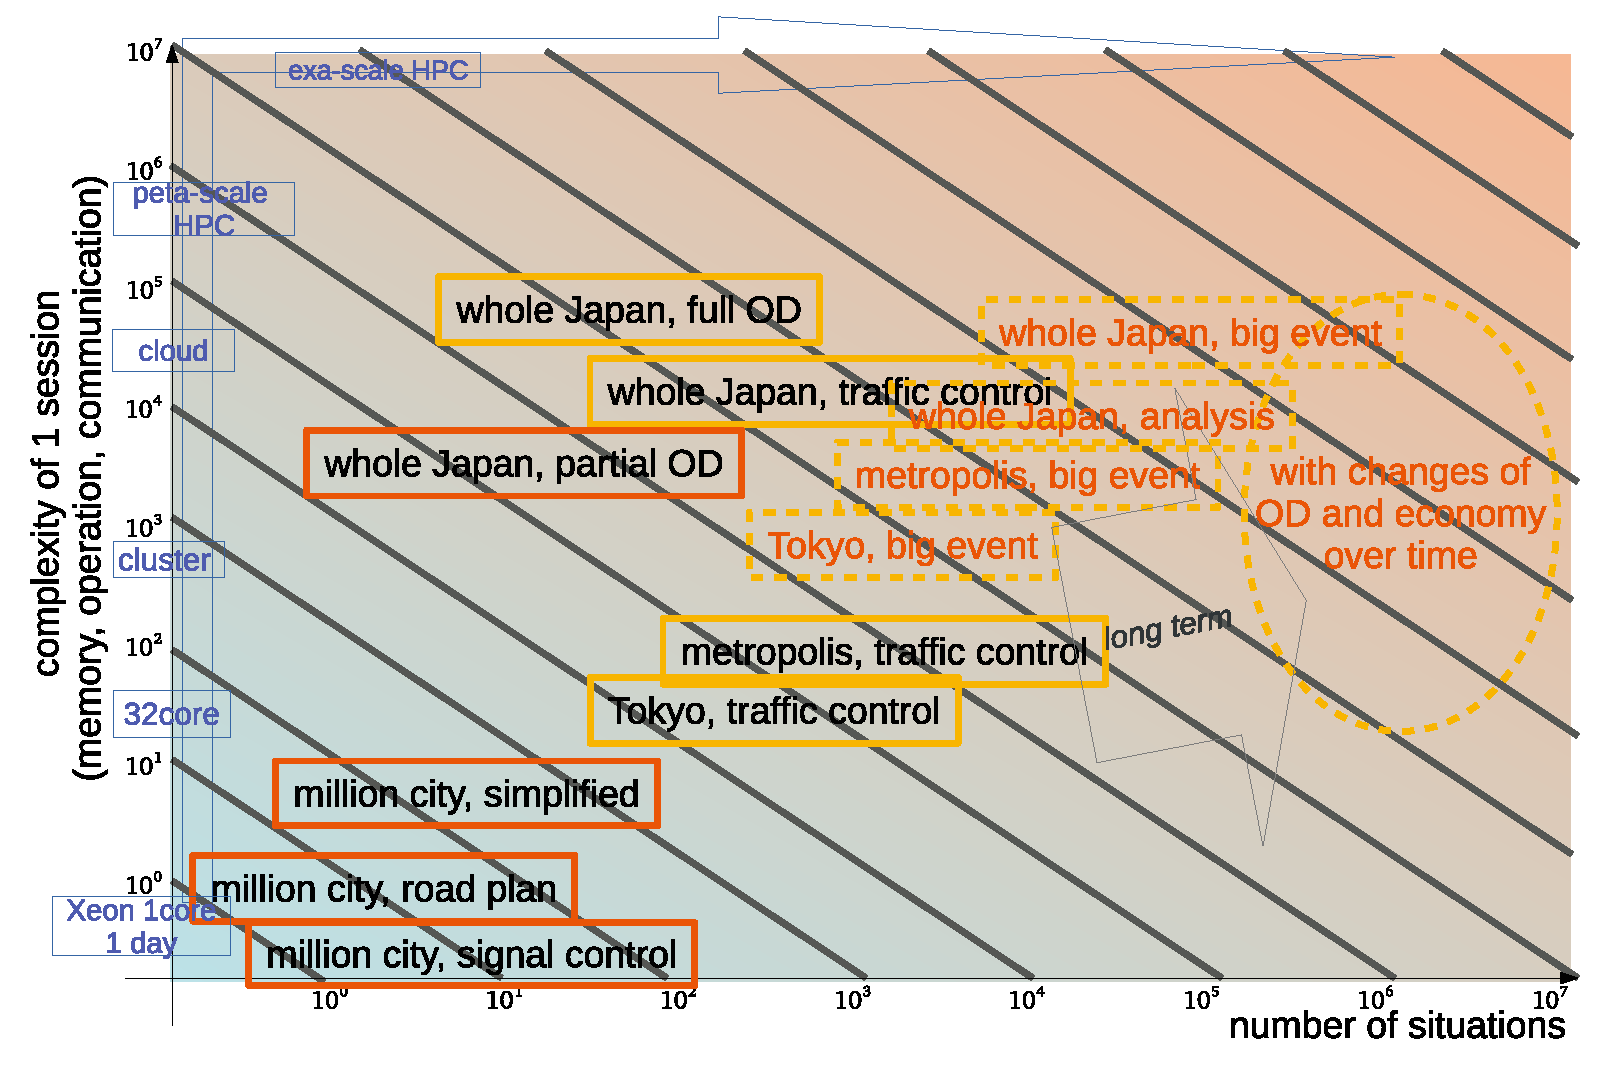
\includegraphics[width=.60\linewidth]{Figs.noda/figure2-5.eps}
  \caption{Roadmap of Traffic Simulation}
  \label{fig:Figure-5}
\end{figure}
%%----------------------------------------------------------------------


%%--------------------------------------------------
\subsection{Market Simulation}
%% - - - - - - - - - - - - - - - - - - - - - - - - -

Market simulations are another important application of multiagent
simulations,
in which agents directly affect each other by selling/buying stocks
and/or currencies \cite{Kawakubo2014a}.
Compared with evacuation and traffic simulations,
market simulations are not constrained by physical space.
Therefore, the time cycles of agents' interactions may be quite short.
Moreover, the ways of thinking of agents show large variations.
This means that the market simulations also require huge
computational cost.

As the reference point of the calculation cost in market simulations,
we present the case of ``tic size'' evaluation.
In this scenario, we conducted a simulation of multiple markets
having different tic sizes,
which is the minimum price unit for trading stocks.
Market companies such as Japan Exchange Group internationally compete
with each other by providing attractive services to traders.
A small tic size
is one of such services that  considerably increases cost.
Therefore, such organizations need evaluations of changes to such services in advance.
In collaborative works with Japan Exchange Group, we conducted a
simulation experiment to find key conditions that determine market share
among markets.
In the simulation, we considered the following scenario:
\begin{itemize}
  \item one good in two markets, 1,000 agents, and 10 million cycles
  \item five cases of tic size and 100 simulation runs per case
\end{itemize}
This simulation takes about one day when using a single thread on a Xeon E5 CPU.
As the reference point, we plot this as ``tic size'' in \figref{fig:Figure-6}.

We are considering extending the market simulations to various
applications used for stock market analyses.
For example, it is in the interest of market companies 
to determine ``daily limit'' and ``cut-off'' prices\cite{Mizuta2013a}.
In this case, the simulation must handle 10--20 goods.
Moreover, evaluating the effects of ``arbitrage'' \cite{Kawakubo2014a}, 
which involves trading rather quickly in intervals of milliseconds,
is important from the viewpoint of maintaining sound market conditions.
This will increase the computational cost, as plotted in \figref{fig:Figure-6}.
Another topic is the evaluation of ``Basel Capital Accords'',
which deal with the soundness of banks in markets.
In the present study, we executed the case of three names for the Basel Accords,
but we will extend it to 100 names in the real application.

The evaluation of ``systemic risks of inter-bank network'' is an important issue
in market evaluation.
However, currently, the 
computational cost of a naive simulation exceeds exa-scale HPC.


%%----------------------------------------------------------------------
\begin{figure}
  \centering
  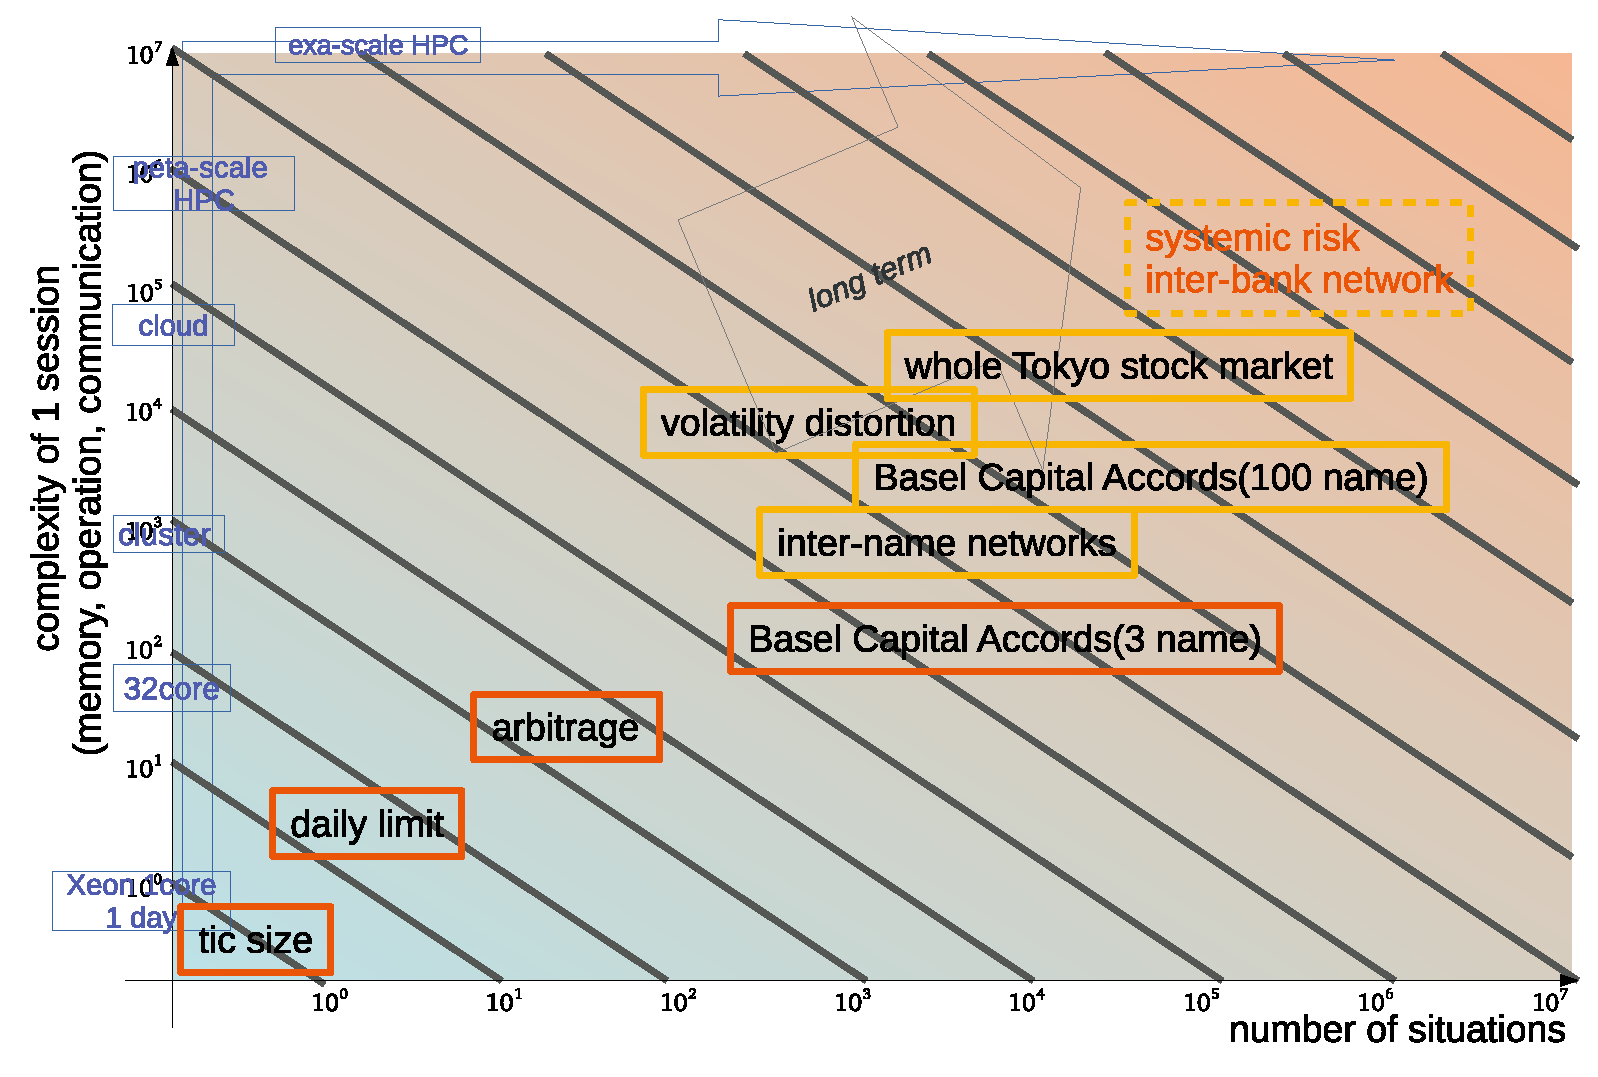
\includegraphics[width=.60\linewidth]{Figs.noda/figure2-6.eps}
  \caption{Roadmap of Market Simulation}
  \label{fig:Figure-6}
\end{figure}
%%----------------------------------------------------------------------

% %%--------------------------------------------------
% \subsection{Transportation Service Simulation}
% %% - - - - - - - - - - - - - - - - - - - - - - - - -
% %%----------------------------------------------------------------------
% \begin{figure}
%   \centering
%   \includegraphics[width=.60\linewidth]{Figs.noda/Figure-8.eps}
%   \caption{Roadmap of Transportation Service Simulation}
%   \label{fig:Figure-8}
% \end{figure}
% %%----------------------------------------------------------------------


%\cite{Noda2013l}



%\bibliographystyle{spbasic}
\bibliographystyle{spmpsci}
\bibliography{main,mizuta-crest,matsushima}
